% Created by tikzDevice version 0.12.6 on 2025-08-29 17:53:08
% !TEX encoding = UTF-8 Unicode
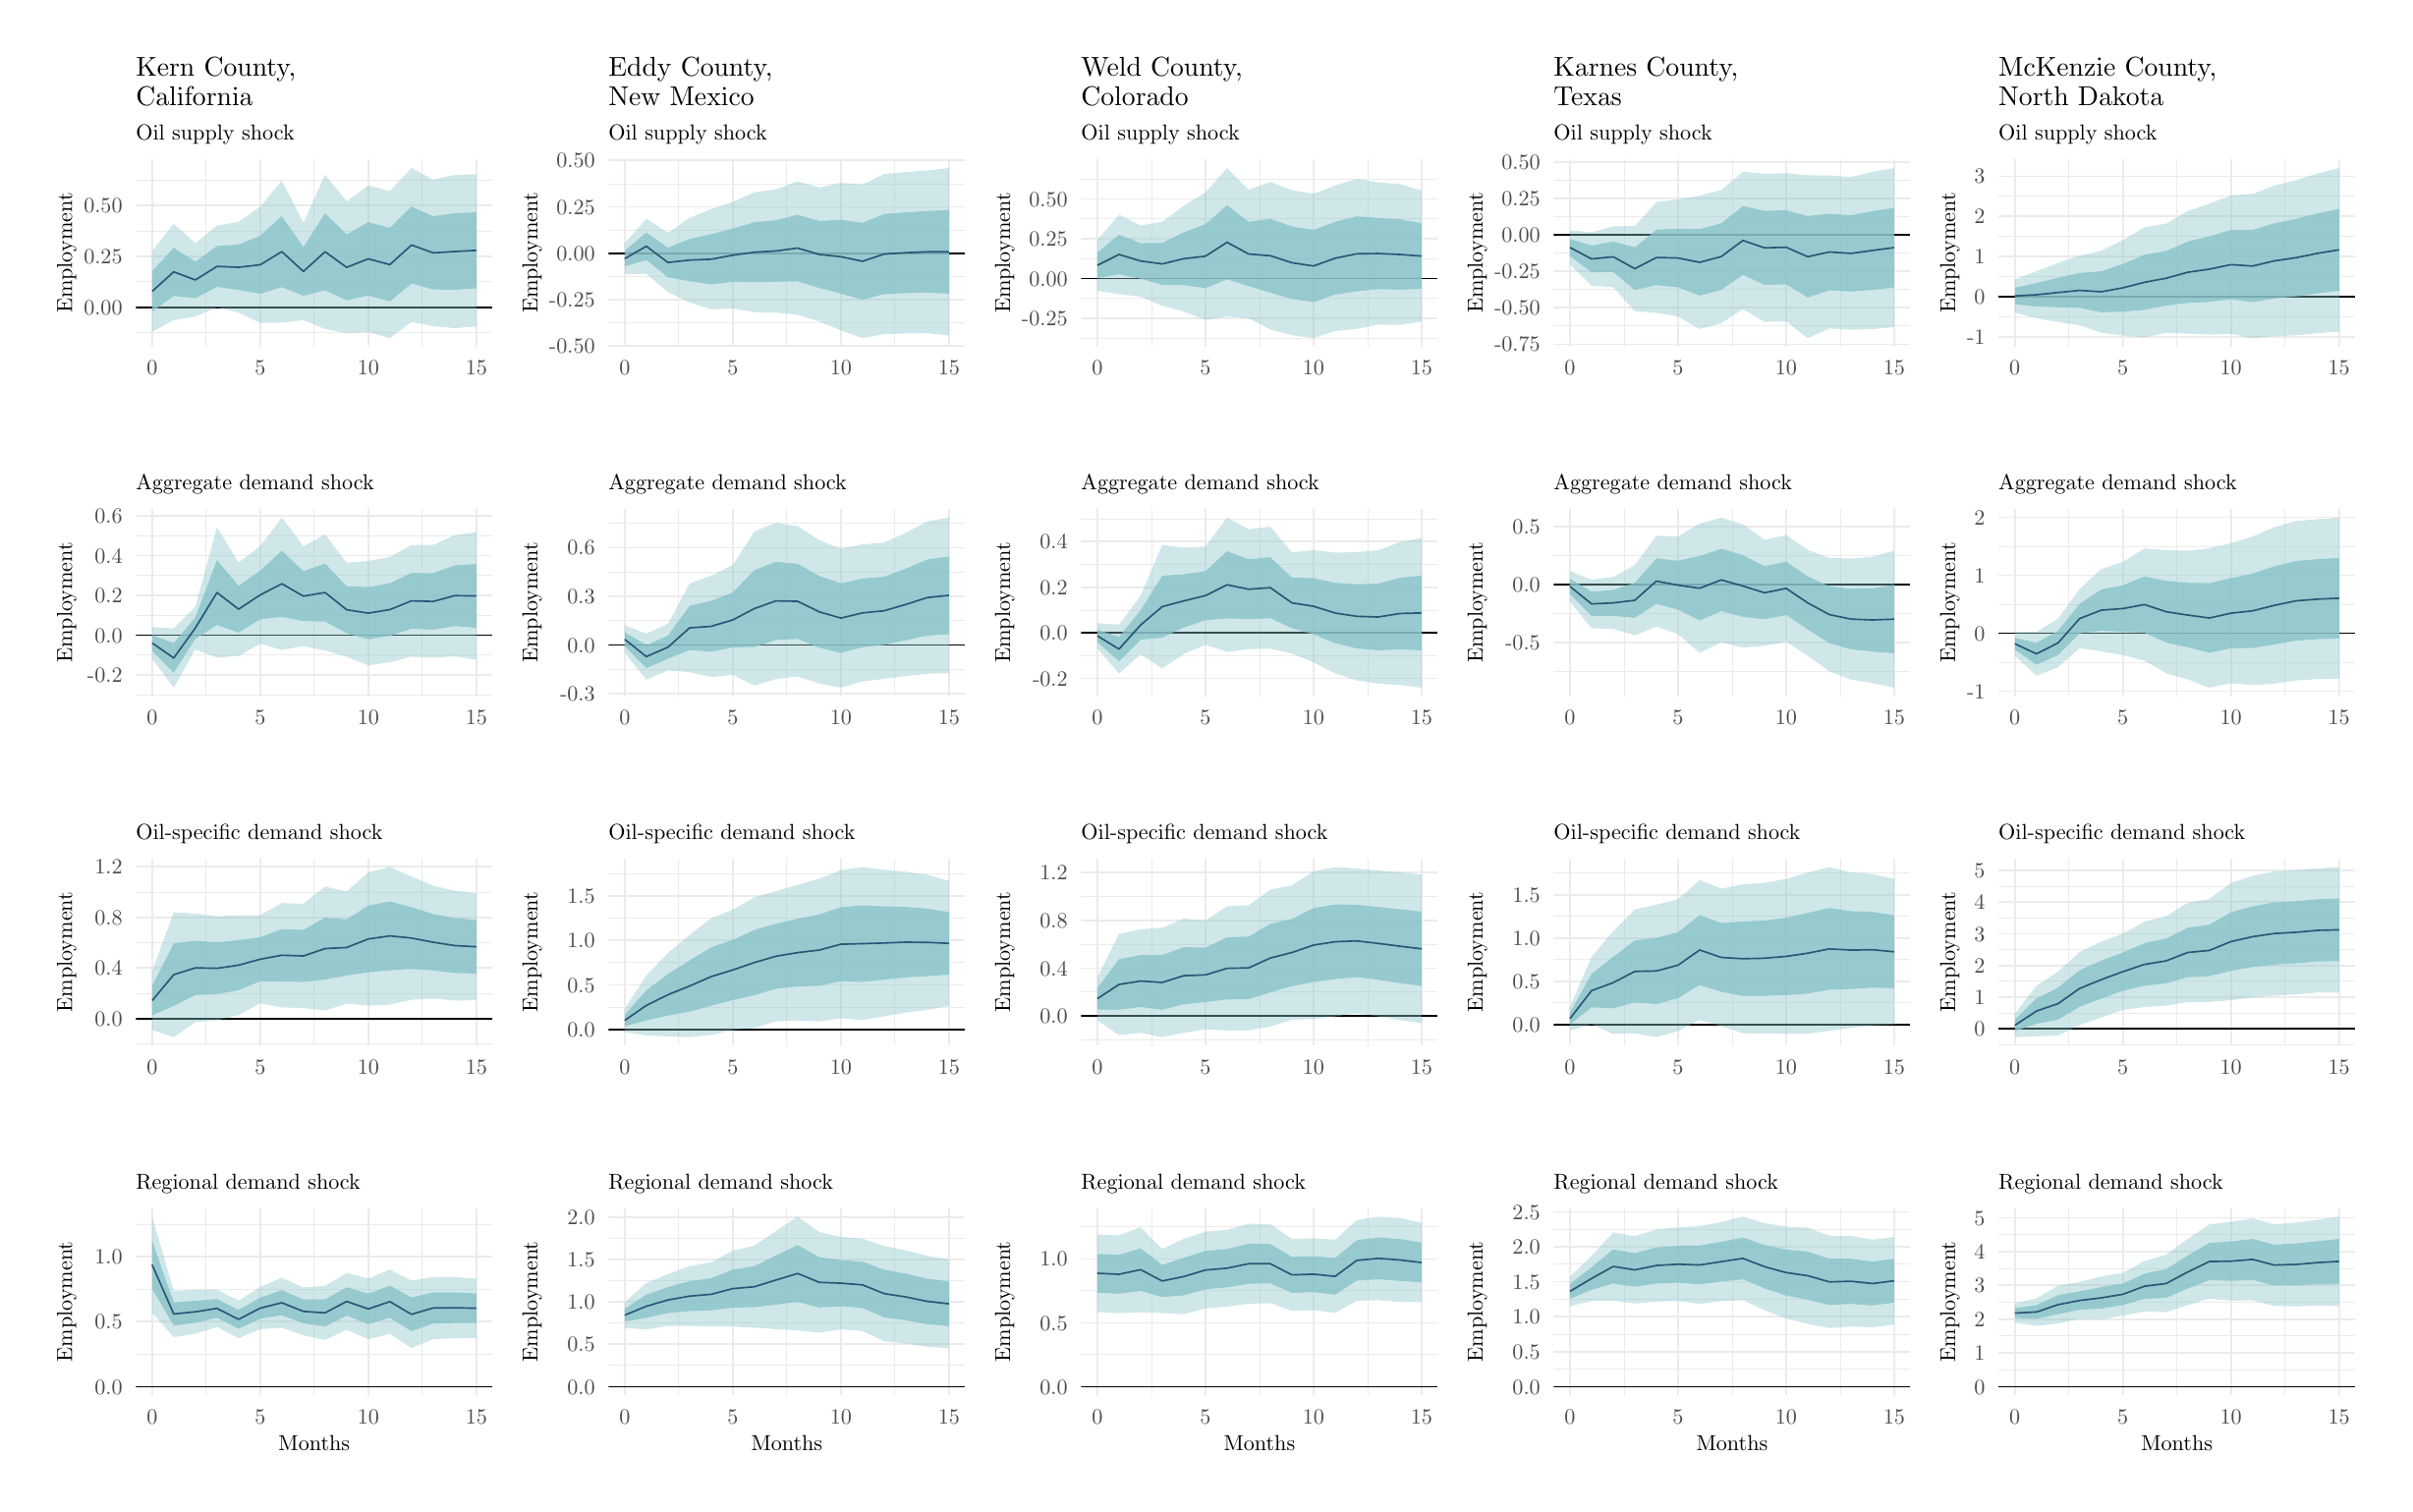
\begin{tikzpicture}[x=1pt,y=1pt]
\definecolor{fillColor}{RGB}{255,255,255}
\path[use as bounding box,fill=fillColor,fill opacity=0.00] (0,0) rectangle (867.24,535.98);
\begin{scope}
\path[clip] ( 39.98,418.47) rectangle (171.16,487.29);
\definecolor{drawColor}{gray}{0.92}

\path[draw=drawColor,line width= 0.3pt,line join=round] ( 39.98,423.59) --
	(171.16,423.59);

\path[draw=drawColor,line width= 0.3pt,line join=round] ( 39.98,442.33) --
	(171.16,442.33);

\path[draw=drawColor,line width= 0.3pt,line join=round] ( 39.98,461.07) --
	(171.16,461.07);

\path[draw=drawColor,line width= 0.3pt,line join=round] ( 39.98,479.82) --
	(171.16,479.82);

\path[draw=drawColor,line width= 0.3pt,line join=round] ( 65.82,418.47) --
	( 65.82,487.29);

\path[draw=drawColor,line width= 0.3pt,line join=round] (105.57,418.47) --
	(105.57,487.29);

\path[draw=drawColor,line width= 0.3pt,line join=round] (145.32,418.47) --
	(145.32,487.29);

\path[draw=drawColor,line width= 0.6pt,line join=round] ( 39.98,432.96) --
	(171.16,432.96);

\path[draw=drawColor,line width= 0.6pt,line join=round] ( 39.98,451.70) --
	(171.16,451.70);

\path[draw=drawColor,line width= 0.6pt,line join=round] ( 39.98,470.45) --
	(171.16,470.45);

\path[draw=drawColor,line width= 0.6pt,line join=round] ( 45.95,418.47) --
	( 45.95,487.29);

\path[draw=drawColor,line width= 0.6pt,line join=round] ( 85.70,418.47) --
	( 85.70,487.29);

\path[draw=drawColor,line width= 0.6pt,line join=round] (125.45,418.47) --
	(125.45,487.29);

\path[draw=drawColor,line width= 0.6pt,line join=round] (165.20,418.47) --
	(165.20,487.29);
\definecolor{drawColor}{RGB}{0,0,0}

\path[draw=drawColor,line width= 0.6pt,line join=round] ( 39.98,432.96) -- (171.16,432.96);
\definecolor{fillColor}{RGB}{136,195,200}

\path[fill=fillColor,fill opacity=0.40] ( 45.95,453.73) --
	( 53.90,463.68) --
	( 61.85,456.50) --
	( 69.80,463.01) --
	( 77.75,464.37) --
	( 85.70,469.95) --
	( 93.65,479.55) --
	(101.60,464.02) --
	(109.55,481.77) --
	(117.50,471.87) --
	(125.45,477.74) --
	(133.40,475.70) --
	(141.35,484.16) --
	(149.30,479.90) --
	(157.25,481.64) --
	(165.20,481.88) --
	(165.20,425.91) --
	(157.25,425.27) --
	(149.30,426.04) --
	(141.35,427.55) --
	(133.40,421.60) --
	(125.45,423.80) --
	(117.50,423.40) --
	(109.55,424.99) --
	(101.60,428.27) --
	( 93.65,427.29) --
	( 85.70,427.21) --
	( 77.75,430.97) --
	( 69.80,432.97) --
	( 61.85,429.52) --
	( 53.90,428.28) --
	( 45.95,423.90) --
	cycle;

\path[] ( 45.95,453.73) --
	( 53.90,463.68) --
	( 61.85,456.50) --
	( 69.80,463.01) --
	( 77.75,464.37) --
	( 85.70,469.95) --
	( 93.65,479.55) --
	(101.60,464.02) --
	(109.55,481.77) --
	(117.50,471.87) --
	(125.45,477.74) --
	(133.40,475.70) --
	(141.35,484.16) --
	(149.30,479.90) --
	(157.25,481.64) --
	(165.20,481.88);

\path[] (165.20,425.91) --
	(157.25,425.27) --
	(149.30,426.04) --
	(141.35,427.55) --
	(133.40,421.60) --
	(125.45,423.80) --
	(117.50,423.40) --
	(109.55,424.99) --
	(101.60,428.27) --
	( 93.65,427.29) --
	( 85.70,427.21) --
	( 77.75,430.97) --
	( 69.80,432.97) --
	( 61.85,429.52) --
	( 53.90,428.28) --
	( 45.95,423.90);
\definecolor{fillColor}{RGB}{136,195,200}

\path[fill=fillColor,fill opacity=0.80] ( 45.95,446.27) --
	( 53.90,454.83) --
	( 61.85,449.76) --
	( 69.80,455.50) --
	( 77.75,456.02) --
	( 85.70,459.27) --
	( 93.65,466.49) --
	(101.60,455.08) --
	(109.55,467.57) --
	(117.50,459.75) --
	(125.45,464.26) --
	(133.40,462.17) --
	(141.35,470.01) --
	(149.30,466.44) --
	(157.25,467.55) --
	(165.20,467.89) --
	(165.20,439.90) --
	(157.25,439.36) --
	(149.30,439.51) --
	(141.35,441.70) --
	(133.40,435.12) --
	(125.45,437.29) --
	(117.50,435.52) --
	(109.55,439.19) --
	(101.60,437.21) --
	( 93.65,440.36) --
	( 85.70,437.90) --
	( 77.75,439.32) --
	( 69.80,440.48) --
	( 61.85,436.27) --
	( 53.90,437.13) --
	( 45.95,431.36) --
	cycle;

\path[] ( 45.95,446.27) --
	( 53.90,454.83) --
	( 61.85,449.76) --
	( 69.80,455.50) --
	( 77.75,456.02) --
	( 85.70,459.27) --
	( 93.65,466.49) --
	(101.60,455.08) --
	(109.55,467.57) --
	(117.50,459.75) --
	(125.45,464.26) --
	(133.40,462.17) --
	(141.35,470.01) --
	(149.30,466.44) --
	(157.25,467.55) --
	(165.20,467.89);

\path[] (165.20,439.90) --
	(157.25,439.36) --
	(149.30,439.51) --
	(141.35,441.70) --
	(133.40,435.12) --
	(125.45,437.29) --
	(117.50,435.52) --
	(109.55,439.19) --
	(101.60,437.21) --
	( 93.65,440.36) --
	( 85.70,437.90) --
	( 77.75,439.32) --
	( 69.80,440.48) --
	( 61.85,436.27) --
	( 53.90,437.13) --
	( 45.95,431.36);
\definecolor{drawColor}{RGB}{42,86,118}

\path[draw=drawColor,line width= 0.6pt,line join=round] ( 45.95,438.81) --
	( 53.90,445.98) --
	( 61.85,443.01) --
	( 69.80,447.99) --
	( 77.75,447.67) --
	( 85.70,448.58) --
	( 93.65,453.42) --
	(101.60,446.14) --
	(109.55,453.38) --
	(117.50,447.64) --
	(125.45,450.77) --
	(133.40,448.65) --
	(141.35,455.86) --
	(149.30,452.97) --
	(157.25,453.45) --
	(165.20,453.89);
\end{scope}
\begin{scope}
\path[clip] (  0.00,  0.00) rectangle (867.24,535.98);
\definecolor{drawColor}{gray}{0.30}

\node[text=drawColor,anchor=base east,inner sep=0pt, outer sep=0pt, scale=  0.80] at ( 35.03,430.21) {0.00};

\node[text=drawColor,anchor=base east,inner sep=0pt, outer sep=0pt, scale=  0.80] at ( 35.03,448.95) {0.25};

\node[text=drawColor,anchor=base east,inner sep=0pt, outer sep=0pt, scale=  0.80] at ( 35.03,467.69) {0.50};
\end{scope}
\begin{scope}
\path[clip] (  0.00,  0.00) rectangle (867.24,535.98);
\definecolor{drawColor}{gray}{0.30}

\node[text=drawColor,anchor=base,inner sep=0pt, outer sep=0pt, scale=  0.80] at ( 45.95,408.01) {0};

\node[text=drawColor,anchor=base,inner sep=0pt, outer sep=0pt, scale=  0.80] at ( 85.70,408.01) {5};

\node[text=drawColor,anchor=base,inner sep=0pt, outer sep=0pt, scale=  0.80] at (125.45,408.01) {10};

\node[text=drawColor,anchor=base,inner sep=0pt, outer sep=0pt, scale=  0.80] at (165.20,408.01) {15};
\end{scope}
\begin{scope}
\path[clip] (  0.00,  0.00) rectangle (867.24,535.98);
\definecolor{drawColor}{RGB}{0,0,0}

\node[text=drawColor,rotate= 90.00,anchor=base,inner sep=0pt, outer sep=0pt, scale=  0.80] at ( 16.51,452.88) {Employment};
\end{scope}
\begin{scope}
\path[clip] (  0.00,  0.00) rectangle (867.24,535.98);
\definecolor{drawColor}{RGB}{0,0,0}

\node[text=drawColor,anchor=base west,inner sep=0pt, outer sep=0pt, scale=  0.80] at ( 39.98,494.34) {Oil supply shock};
\end{scope}
\begin{scope}
\path[clip] (  0.00,  0.00) rectangle (867.24,535.98);
\definecolor{drawColor}{RGB}{0,0,0}

\node[text=drawColor,anchor=base west,inner sep=0pt, outer sep=0pt, scale=  1.00] at ( 39.98,518.10) {Kern County,};

\node[text=drawColor,anchor=base west,inner sep=0pt, outer sep=0pt, scale=  1.00] at ( 39.98,507.30) {California };
\end{scope}
\begin{scope}
\path[clip] ( 39.98,289.92) rectangle (171.16,358.74);
\definecolor{drawColor}{gray}{0.92}

\path[draw=drawColor,line width= 0.3pt,line join=round] ( 39.98,290.43) --
	(171.16,290.43);

\path[draw=drawColor,line width= 0.3pt,line join=round] ( 39.98,305.07) --
	(171.16,305.07);

\path[draw=drawColor,line width= 0.3pt,line join=round] ( 39.98,319.71) --
	(171.16,319.71);

\path[draw=drawColor,line width= 0.3pt,line join=round] ( 39.98,334.35) --
	(171.16,334.35);

\path[draw=drawColor,line width= 0.3pt,line join=round] ( 39.98,348.99) --
	(171.16,348.99);

\path[draw=drawColor,line width= 0.3pt,line join=round] ( 65.82,289.92) --
	( 65.82,358.74);

\path[draw=drawColor,line width= 0.3pt,line join=round] (105.57,289.92) --
	(105.57,358.74);

\path[draw=drawColor,line width= 0.3pt,line join=round] (145.32,289.92) --
	(145.32,358.74);

\path[draw=drawColor,line width= 0.6pt,line join=round] ( 39.98,297.75) --
	(171.16,297.75);

\path[draw=drawColor,line width= 0.6pt,line join=round] ( 39.98,312.39) --
	(171.16,312.39);

\path[draw=drawColor,line width= 0.6pt,line join=round] ( 39.98,327.03) --
	(171.16,327.03);

\path[draw=drawColor,line width= 0.6pt,line join=round] ( 39.98,341.67) --
	(171.16,341.67);

\path[draw=drawColor,line width= 0.6pt,line join=round] ( 39.98,356.31) --
	(171.16,356.31);

\path[draw=drawColor,line width= 0.6pt,line join=round] ( 45.95,289.92) --
	( 45.95,358.74);

\path[draw=drawColor,line width= 0.6pt,line join=round] ( 85.70,289.92) --
	( 85.70,358.74);

\path[draw=drawColor,line width= 0.6pt,line join=round] (125.45,289.92) --
	(125.45,358.74);

\path[draw=drawColor,line width= 0.6pt,line join=round] (165.20,289.92) --
	(165.20,358.74);
\definecolor{drawColor}{RGB}{0,0,0}

\path[draw=drawColor,line width= 0.6pt,line join=round] ( 39.98,312.39) -- (171.16,312.39);
\definecolor{fillColor}{RGB}{136,195,200}

\path[fill=fillColor,fill opacity=0.40] ( 45.95,315.32) --
	( 53.90,314.87) --
	( 61.85,322.88) --
	( 69.80,351.97) --
	( 77.75,339.09) --
	( 85.70,345.07) --
	( 93.65,355.61) --
	(101.60,345.07) --
	(109.55,349.40) --
	(117.50,339.04) --
	(125.45,339.66) --
	(133.40,341.11) --
	(141.35,345.51) --
	(149.30,345.54) --
	(157.25,349.19) --
	(165.20,350.24) --
	(165.20,303.31) --
	(157.25,304.60) --
	(149.30,303.98) --
	(141.35,304.46) --
	(133.40,302.42) --
	(125.45,301.26) --
	(117.50,304.38) --
	(109.55,306.70) --
	(101.60,308.37) --
	( 93.65,306.91) --
	( 85.70,309.24) --
	( 77.75,304.72) --
	( 69.80,304.11) --
	( 61.85,307.11) --
	( 53.90,293.05) --
	( 45.95,303.66) --
	cycle;

\path[] ( 45.95,315.32) --
	( 53.90,314.87) --
	( 61.85,322.88) --
	( 69.80,351.97) --
	( 77.75,339.09) --
	( 85.70,345.07) --
	( 93.65,355.61) --
	(101.60,345.07) --
	(109.55,349.40) --
	(117.50,339.04) --
	(125.45,339.66) --
	(133.40,341.11) --
	(141.35,345.51) --
	(149.30,345.54) --
	(157.25,349.19) --
	(165.20,350.24);

\path[] (165.20,303.31) --
	(157.25,304.60) --
	(149.30,303.98) --
	(141.35,304.46) --
	(133.40,302.42) --
	(125.45,301.26) --
	(117.50,304.38) --
	(109.55,306.70) --
	(101.60,308.37) --
	( 93.65,306.91) --
	( 85.70,309.24) --
	( 77.75,304.72) --
	( 69.80,304.11) --
	( 61.85,307.11) --
	( 53.90,293.05) --
	( 45.95,303.66);
\definecolor{fillColor}{RGB}{136,195,200}

\path[fill=fillColor,fill opacity=0.80] ( 45.95,312.40) --
	( 53.90,309.41) --
	( 61.85,318.93) --
	( 69.80,340.01) --
	( 77.75,330.50) --
	( 85.70,336.12) --
	( 93.65,343.44) --
	(101.60,335.90) --
	(109.55,338.72) --
	(117.50,330.37) --
	(125.45,330.06) --
	(133.40,331.44) --
	(141.35,335.25) --
	(149.30,335.15) --
	(157.25,338.04) --
	(165.20,338.51) --
	(165.20,315.04) --
	(157.25,315.75) --
	(149.30,314.37) --
	(141.35,314.72) --
	(133.40,312.09) --
	(125.45,310.86) --
	(117.50,313.05) --
	(109.55,317.37) --
	(101.60,317.55) --
	( 93.65,319.09) --
	( 85.70,318.20) --
	( 77.75,313.31) --
	( 69.80,316.08) --
	( 61.85,311.05) --
	( 53.90,298.50) --
	( 45.95,306.57) --
	cycle;

\path[] ( 45.95,312.40) --
	( 53.90,309.41) --
	( 61.85,318.93) --
	( 69.80,340.01) --
	( 77.75,330.50) --
	( 85.70,336.12) --
	( 93.65,343.44) --
	(101.60,335.90) --
	(109.55,338.72) --
	(117.50,330.37) --
	(125.45,330.06) --
	(133.40,331.44) --
	(141.35,335.25) --
	(149.30,335.15) --
	(157.25,338.04) --
	(165.20,338.51);

\path[] (165.20,315.04) --
	(157.25,315.75) --
	(149.30,314.37) --
	(141.35,314.72) --
	(133.40,312.09) --
	(125.45,310.86) --
	(117.50,313.05) --
	(109.55,317.37) --
	(101.60,317.55) --
	( 93.65,319.09) --
	( 85.70,318.20) --
	( 77.75,313.31) --
	( 69.80,316.08) --
	( 61.85,311.05) --
	( 53.90,298.50) --
	( 45.95,306.57);
\definecolor{drawColor}{RGB}{42,86,118}

\path[draw=drawColor,line width= 0.6pt,line join=round] ( 45.95,309.49) --
	( 53.90,303.96) --
	( 61.85,314.99) --
	( 69.80,328.04) --
	( 77.75,321.91) --
	( 85.70,327.16) --
	( 93.65,331.26) --
	(101.60,326.72) --
	(109.55,328.05) --
	(117.50,321.71) --
	(125.45,320.46) --
	(133.40,321.76) --
	(141.35,324.98) --
	(149.30,324.76) --
	(157.25,326.90) --
	(165.20,326.78);
\end{scope}
\begin{scope}
\path[clip] (  0.00,  0.00) rectangle (867.24,535.98);
\definecolor{drawColor}{gray}{0.30}

\node[text=drawColor,anchor=base east,inner sep=0pt, outer sep=0pt, scale=  0.80] at ( 35.03,294.99) {-0.2};

\node[text=drawColor,anchor=base east,inner sep=0pt, outer sep=0pt, scale=  0.80] at ( 35.03,309.63) {0.0};

\node[text=drawColor,anchor=base east,inner sep=0pt, outer sep=0pt, scale=  0.80] at ( 35.03,324.27) {0.2};

\node[text=drawColor,anchor=base east,inner sep=0pt, outer sep=0pt, scale=  0.80] at ( 35.03,338.91) {0.4};

\node[text=drawColor,anchor=base east,inner sep=0pt, outer sep=0pt, scale=  0.80] at ( 35.03,353.55) {0.6};
\end{scope}
\begin{scope}
\path[clip] (  0.00,  0.00) rectangle (867.24,535.98);
\definecolor{drawColor}{gray}{0.30}

\node[text=drawColor,anchor=base,inner sep=0pt, outer sep=0pt, scale=  0.80] at ( 45.95,279.46) {0};

\node[text=drawColor,anchor=base,inner sep=0pt, outer sep=0pt, scale=  0.80] at ( 85.70,279.46) {5};

\node[text=drawColor,anchor=base,inner sep=0pt, outer sep=0pt, scale=  0.80] at (125.45,279.46) {10};

\node[text=drawColor,anchor=base,inner sep=0pt, outer sep=0pt, scale=  0.80] at (165.20,279.46) {15};
\end{scope}
\begin{scope}
\path[clip] (  0.00,  0.00) rectangle (867.24,535.98);
\definecolor{drawColor}{RGB}{0,0,0}

\node[text=drawColor,rotate= 90.00,anchor=base,inner sep=0pt, outer sep=0pt, scale=  0.80] at ( 16.51,324.33) {Employment};
\end{scope}
\begin{scope}
\path[clip] (  0.00,  0.00) rectangle (867.24,535.98);
\definecolor{drawColor}{RGB}{0,0,0}

\node[text=drawColor,anchor=base west,inner sep=0pt, outer sep=0pt, scale=  0.80] at ( 39.98,365.80) {Aggregate demand shock};
\end{scope}
\begin{scope}
\path[clip] ( 39.98,161.38) rectangle (171.16,230.20);
\definecolor{drawColor}{gray}{0.92}

\path[draw=drawColor,line width= 0.3pt,line join=round] ( 39.98,161.98) --
	(171.16,161.98);

\path[draw=drawColor,line width= 0.3pt,line join=round] ( 39.98,180.61) --
	(171.16,180.61);

\path[draw=drawColor,line width= 0.3pt,line join=round] ( 39.98,199.25) --
	(171.16,199.25);

\path[draw=drawColor,line width= 0.3pt,line join=round] ( 39.98,217.89) --
	(171.16,217.89);

\path[draw=drawColor,line width= 0.3pt,line join=round] ( 65.82,161.38) --
	( 65.82,230.20);

\path[draw=drawColor,line width= 0.3pt,line join=round] (105.57,161.38) --
	(105.57,230.20);

\path[draw=drawColor,line width= 0.3pt,line join=round] (145.32,161.38) --
	(145.32,230.20);

\path[draw=drawColor,line width= 0.6pt,line join=round] ( 39.98,171.29) --
	(171.16,171.29);

\path[draw=drawColor,line width= 0.6pt,line join=round] ( 39.98,189.93) --
	(171.16,189.93);

\path[draw=drawColor,line width= 0.6pt,line join=round] ( 39.98,208.57) --
	(171.16,208.57);

\path[draw=drawColor,line width= 0.6pt,line join=round] ( 39.98,227.21) --
	(171.16,227.21);

\path[draw=drawColor,line width= 0.6pt,line join=round] ( 45.95,161.38) --
	( 45.95,230.20);

\path[draw=drawColor,line width= 0.6pt,line join=round] ( 85.70,161.38) --
	( 85.70,230.20);

\path[draw=drawColor,line width= 0.6pt,line join=round] (125.45,161.38) --
	(125.45,230.20);

\path[draw=drawColor,line width= 0.6pt,line join=round] (165.20,161.38) --
	(165.20,230.20);
\definecolor{drawColor}{RGB}{0,0,0}

\path[draw=drawColor,line width= 0.6pt,line join=round] ( 39.98,171.29) -- (171.16,171.29);
\definecolor{fillColor}{RGB}{136,195,200}

\path[fill=fillColor,fill opacity=0.40] ( 45.95,188.75) --
	( 53.90,210.46) --
	( 61.85,209.99) --
	( 69.80,208.92) --
	( 77.75,209.37) --
	( 85.70,209.36) --
	( 93.65,213.83) --
	(101.60,213.53) --
	(109.55,219.88) --
	(117.50,218.11) --
	(125.45,225.14) --
	(133.40,227.07) --
	(141.35,223.63) --
	(149.30,220.19) --
	(157.25,218.38) --
	(165.20,217.46) --
	(165.20,178.05) --
	(157.25,178.00) --
	(149.30,178.66) --
	(141.35,178.26) --
	(133.40,176.46) --
	(125.45,176.10) --
	(117.50,176.85) --
	(109.55,174.29) --
	(101.60,175.21) --
	( 93.65,175.45) --
	( 85.70,176.98) --
	( 77.75,172.59) --
	( 69.80,170.74) --
	( 61.85,170.00) --
	( 53.90,164.50) --
	( 45.95,167.14) --
	cycle;

\path[] ( 45.95,188.75) --
	( 53.90,210.46) --
	( 61.85,209.99) --
	( 69.80,208.92) --
	( 77.75,209.37) --
	( 85.70,209.36) --
	( 93.65,213.83) --
	(101.60,213.53) --
	(109.55,219.88) --
	(117.50,218.11) --
	(125.45,225.14) --
	(133.40,227.07) --
	(141.35,223.63) --
	(149.30,220.19) --
	(157.25,218.38) --
	(165.20,217.46);

\path[] (165.20,178.05) --
	(157.25,178.00) --
	(149.30,178.66) --
	(141.35,178.26) --
	(133.40,176.46) --
	(125.45,176.10) --
	(117.50,176.85) --
	(109.55,174.29) --
	(101.60,175.21) --
	( 93.65,175.45) --
	( 85.70,176.98) --
	( 77.75,172.59) --
	( 69.80,170.74) --
	( 61.85,170.00) --
	( 53.90,164.50) --
	( 45.95,167.14);
\definecolor{fillColor}{RGB}{136,195,200}

\path[fill=fillColor,fill opacity=0.80] ( 45.95,183.35) --
	( 53.90,198.97) --
	( 61.85,199.99) --
	( 69.80,199.37) --
	( 77.75,200.18) --
	( 85.70,201.26) --
	( 93.65,204.23) --
	(101.60,203.95) --
	(109.55,208.48) --
	(117.50,207.80) --
	(125.45,212.88) --
	(133.40,214.42) --
	(141.35,212.29) --
	(149.30,209.81) --
	(157.25,208.29) --
	(165.20,207.60) --
	(165.20,187.90) --
	(157.25,188.10) --
	(149.30,189.05) --
	(141.35,189.60) --
	(133.40,189.11) --
	(125.45,188.36) --
	(117.50,187.17) --
	(109.55,185.69) --
	(101.60,184.79) --
	( 93.65,185.04) --
	( 85.70,185.08) --
	( 77.75,181.79) --
	( 69.80,180.28) --
	( 61.85,180.00) --
	( 53.90,175.99) --
	( 45.95,172.54) --
	cycle;

\path[] ( 45.95,183.35) --
	( 53.90,198.97) --
	( 61.85,199.99) --
	( 69.80,199.37) --
	( 77.75,200.18) --
	( 85.70,201.26) --
	( 93.65,204.23) --
	(101.60,203.95) --
	(109.55,208.48) --
	(117.50,207.80) --
	(125.45,212.88) --
	(133.40,214.42) --
	(141.35,212.29) --
	(149.30,209.81) --
	(157.25,208.29) --
	(165.20,207.60);

\path[] (165.20,187.90) --
	(157.25,188.10) --
	(149.30,189.05) --
	(141.35,189.60) --
	(133.40,189.11) --
	(125.45,188.36) --
	(117.50,187.17) --
	(109.55,185.69) --
	(101.60,184.79) --
	( 93.65,185.04) --
	( 85.70,185.08) --
	( 77.75,181.79) --
	( 69.80,180.28) --
	( 61.85,180.00) --
	( 53.90,175.99) --
	( 45.95,172.54);
\definecolor{drawColor}{RGB}{42,86,118}

\path[draw=drawColor,line width= 0.6pt,line join=round] ( 45.95,177.95) --
	( 53.90,187.48) --
	( 61.85,190.00) --
	( 69.80,189.83) --
	( 77.75,190.98) --
	( 85.70,193.17) --
	( 93.65,194.64) --
	(101.60,194.37) --
	(109.55,197.09) --
	(117.50,197.48) --
	(125.45,200.62) --
	(133.40,201.76) --
	(141.35,200.95) --
	(149.30,199.43) --
	(157.25,198.19) --
	(165.20,197.75);
\end{scope}
\begin{scope}
\path[clip] (  0.00,  0.00) rectangle (867.24,535.98);
\definecolor{drawColor}{gray}{0.30}

\node[text=drawColor,anchor=base east,inner sep=0pt, outer sep=0pt, scale=  0.80] at ( 35.03,168.54) {0.0};

\node[text=drawColor,anchor=base east,inner sep=0pt, outer sep=0pt, scale=  0.80] at ( 35.03,187.18) {0.4};

\node[text=drawColor,anchor=base east,inner sep=0pt, outer sep=0pt, scale=  0.80] at ( 35.03,205.81) {0.8};

\node[text=drawColor,anchor=base east,inner sep=0pt, outer sep=0pt, scale=  0.80] at ( 35.03,224.45) {1.2};
\end{scope}
\begin{scope}
\path[clip] (  0.00,  0.00) rectangle (867.24,535.98);
\definecolor{drawColor}{gray}{0.30}

\node[text=drawColor,anchor=base,inner sep=0pt, outer sep=0pt, scale=  0.80] at ( 45.95,150.92) {0};

\node[text=drawColor,anchor=base,inner sep=0pt, outer sep=0pt, scale=  0.80] at ( 85.70,150.92) {5};

\node[text=drawColor,anchor=base,inner sep=0pt, outer sep=0pt, scale=  0.80] at (125.45,150.92) {10};

\node[text=drawColor,anchor=base,inner sep=0pt, outer sep=0pt, scale=  0.80] at (165.20,150.92) {15};
\end{scope}
\begin{scope}
\path[clip] (  0.00,  0.00) rectangle (867.24,535.98);
\definecolor{drawColor}{RGB}{0,0,0}

\node[text=drawColor,rotate= 90.00,anchor=base,inner sep=0pt, outer sep=0pt, scale=  0.80] at ( 16.51,195.79) {Employment};
\end{scope}
\begin{scope}
\path[clip] (  0.00,  0.00) rectangle (867.24,535.98);
\definecolor{drawColor}{RGB}{0,0,0}

\node[text=drawColor,anchor=base west,inner sep=0pt, outer sep=0pt, scale=  0.80] at ( 39.98,237.25) {Oil-specific demand shock};
\end{scope}
\begin{scope}
\path[clip] ( 39.98, 32.83) rectangle (171.16,101.65);
\definecolor{drawColor}{gray}{0.92}

\path[draw=drawColor,line width= 0.3pt,line join=round] ( 39.98, 47.91) --
	(171.16, 47.91);

\path[draw=drawColor,line width= 0.3pt,line join=round] ( 39.98, 71.80) --
	(171.16, 71.80);

\path[draw=drawColor,line width= 0.3pt,line join=round] ( 39.98, 95.70) --
	(171.16, 95.70);

\path[draw=drawColor,line width= 0.3pt,line join=round] ( 65.82, 32.83) --
	( 65.82,101.65);

\path[draw=drawColor,line width= 0.3pt,line join=round] (105.57, 32.83) --
	(105.57,101.65);

\path[draw=drawColor,line width= 0.3pt,line join=round] (145.32, 32.83) --
	(145.32,101.65);

\path[draw=drawColor,line width= 0.6pt,line join=round] ( 39.98, 35.96) --
	(171.16, 35.96);

\path[draw=drawColor,line width= 0.6pt,line join=round] ( 39.98, 59.85) --
	(171.16, 59.85);

\path[draw=drawColor,line width= 0.6pt,line join=round] ( 39.98, 83.75) --
	(171.16, 83.75);

\path[draw=drawColor,line width= 0.6pt,line join=round] ( 45.95, 32.83) --
	( 45.95,101.65);

\path[draw=drawColor,line width= 0.6pt,line join=round] ( 85.70, 32.83) --
	( 85.70,101.65);

\path[draw=drawColor,line width= 0.6pt,line join=round] (125.45, 32.83) --
	(125.45,101.65);

\path[draw=drawColor,line width= 0.6pt,line join=round] (165.20, 32.83) --
	(165.20,101.65);
\definecolor{drawColor}{RGB}{0,0,0}

\path[draw=drawColor,line width= 0.6pt,line join=round] ( 39.98, 35.96) -- (171.16, 35.96);
\definecolor{fillColor}{RGB}{136,195,200}

\path[fill=fillColor,fill opacity=0.40] ( 45.95, 98.52) --
	( 53.90, 71.20) --
	( 61.85, 71.58) --
	( 69.80, 71.62) --
	( 77.75, 67.64) --
	( 85.70, 72.57) --
	( 93.65, 76.06) --
	(101.60, 72.46) --
	(109.55, 73.05) --
	(117.50, 77.75) --
	(125.45, 75.73) --
	(133.40, 79.02) --
	(141.35, 74.96) --
	(149.30, 76.33) --
	(157.25, 76.23) --
	(165.20, 75.73) --
	(165.20, 53.87) --
	(157.25, 53.74) --
	(149.30, 53.47) --
	(141.35, 50.16) --
	(133.40, 55.43) --
	(125.45, 53.38) --
	(117.50, 56.88) --
	(109.55, 53.13) --
	(101.60, 54.84) --
	( 93.65, 57.61) --
	( 85.70, 57.11) --
	( 77.75, 53.78) --
	( 69.80, 57.89) --
	( 61.85, 55.39) --
	( 53.90, 54.17) --
	( 45.95, 63.07) --
	cycle;

\path[] ( 45.95, 98.52) --
	( 53.90, 71.20) --
	( 61.85, 71.58) --
	( 69.80, 71.62) --
	( 77.75, 67.64) --
	( 85.70, 72.57) --
	( 93.65, 76.06) --
	(101.60, 72.46) --
	(109.55, 73.05) --
	(117.50, 77.75) --
	(125.45, 75.73) --
	(133.40, 79.02) --
	(141.35, 74.96) --
	(149.30, 76.33) --
	(157.25, 76.23) --
	(165.20, 75.73);

\path[] (165.20, 53.87) --
	(157.25, 53.74) --
	(149.30, 53.47) --
	(141.35, 50.16) --
	(133.40, 55.43) --
	(125.45, 53.38) --
	(117.50, 56.88) --
	(109.55, 53.13) --
	(101.60, 54.84) --
	( 93.65, 57.61) --
	( 85.70, 57.11) --
	( 77.75, 53.78) --
	( 69.80, 57.89) --
	( 61.85, 55.39) --
	( 53.90, 54.17) --
	( 45.95, 63.07);
\definecolor{fillColor}{RGB}{136,195,200}

\path[fill=fillColor,fill opacity=0.80] ( 45.95, 89.66) --
	( 53.90, 66.95) --
	( 61.85, 67.53) --
	( 69.80, 68.19) --
	( 77.75, 64.18) --
	( 85.70, 68.71) --
	( 93.65, 71.45) --
	(101.60, 68.06) --
	(109.55, 68.07) --
	(117.50, 72.53) --
	(125.45, 70.14) --
	(133.40, 73.12) --
	(141.35, 68.76) --
	(149.30, 70.62) --
	(157.25, 70.60) --
	(165.20, 70.26) --
	(165.20, 59.33) --
	(157.25, 59.36) --
	(149.30, 59.18) --
	(141.35, 56.36) --
	(133.40, 61.33) --
	(125.45, 58.96) --
	(117.50, 62.10) --
	(109.55, 58.11) --
	(101.60, 59.25) --
	( 93.65, 62.22) --
	( 85.70, 60.98) --
	( 77.75, 57.25) --
	( 69.80, 61.32) --
	( 61.85, 59.44) --
	( 53.90, 58.43) --
	( 45.95, 71.93) --
	cycle;

\path[] ( 45.95, 89.66) --
	( 53.90, 66.95) --
	( 61.85, 67.53) --
	( 69.80, 68.19) --
	( 77.75, 64.18) --
	( 85.70, 68.71) --
	( 93.65, 71.45) --
	(101.60, 68.06) --
	(109.55, 68.07) --
	(117.50, 72.53) --
	(125.45, 70.14) --
	(133.40, 73.12) --
	(141.35, 68.76) --
	(149.30, 70.62) --
	(157.25, 70.60) --
	(165.20, 70.26);

\path[] (165.20, 59.33) --
	(157.25, 59.36) --
	(149.30, 59.18) --
	(141.35, 56.36) --
	(133.40, 61.33) --
	(125.45, 58.96) --
	(117.50, 62.10) --
	(109.55, 58.11) --
	(101.60, 59.25) --
	( 93.65, 62.22) --
	( 85.70, 60.98) --
	( 77.75, 57.25) --
	( 69.80, 61.32) --
	( 61.85, 59.44) --
	( 53.90, 58.43) --
	( 45.95, 71.93);
\definecolor{drawColor}{RGB}{42,86,118}

\path[draw=drawColor,line width= 0.6pt,line join=round] ( 45.95, 80.80) --
	( 53.90, 62.69) --
	( 61.85, 63.49) --
	( 69.80, 64.75) --
	( 77.75, 60.71) --
	( 85.70, 64.84) --
	( 93.65, 66.83) --
	(101.60, 63.65) --
	(109.55, 63.09) --
	(117.50, 67.31) --
	(125.45, 64.55) --
	(133.40, 67.23) --
	(141.35, 62.56) --
	(149.30, 64.90) --
	(157.25, 64.98) --
	(165.20, 64.80);
\end{scope}
\begin{scope}
\path[clip] (  0.00,  0.00) rectangle (867.24,535.98);
\definecolor{drawColor}{gray}{0.30}

\node[text=drawColor,anchor=base east,inner sep=0pt, outer sep=0pt, scale=  0.80] at ( 35.03, 33.20) {0.0};

\node[text=drawColor,anchor=base east,inner sep=0pt, outer sep=0pt, scale=  0.80] at ( 35.03, 57.10) {0.5};

\node[text=drawColor,anchor=base east,inner sep=0pt, outer sep=0pt, scale=  0.80] at ( 35.03, 80.99) {1.0};
\end{scope}
\begin{scope}
\path[clip] (  0.00,  0.00) rectangle (867.24,535.98);
\definecolor{drawColor}{gray}{0.30}

\node[text=drawColor,anchor=base,inner sep=0pt, outer sep=0pt, scale=  0.80] at ( 45.95, 22.37) {0};

\node[text=drawColor,anchor=base,inner sep=0pt, outer sep=0pt, scale=  0.80] at ( 85.70, 22.37) {5};

\node[text=drawColor,anchor=base,inner sep=0pt, outer sep=0pt, scale=  0.80] at (125.45, 22.37) {10};

\node[text=drawColor,anchor=base,inner sep=0pt, outer sep=0pt, scale=  0.80] at (165.20, 22.37) {15};
\end{scope}
\begin{scope}
\path[clip] (  0.00,  0.00) rectangle (867.24,535.98);
\definecolor{drawColor}{RGB}{0,0,0}

\node[text=drawColor,anchor=base,inner sep=0pt, outer sep=0pt, scale=  0.80] at (105.57, 12.56) {Months};
\end{scope}
\begin{scope}
\path[clip] (  0.00,  0.00) rectangle (867.24,535.98);
\definecolor{drawColor}{RGB}{0,0,0}

\node[text=drawColor,rotate= 90.00,anchor=base,inner sep=0pt, outer sep=0pt, scale=  0.80] at ( 16.51, 67.24) {Employment};
\end{scope}
\begin{scope}
\path[clip] (  0.00,  0.00) rectangle (867.24,535.98);
\definecolor{drawColor}{RGB}{0,0,0}

\node[text=drawColor,anchor=base west,inner sep=0pt, outer sep=0pt, scale=  0.80] at ( 39.98,108.70) {Regional demand shock};
\end{scope}
\begin{scope}
\path[clip] (213.81,418.47) rectangle (344.98,487.29);
\definecolor{drawColor}{gray}{0.92}

\path[draw=drawColor,line width= 0.3pt,line join=round] (213.81,427.23) --
	(344.98,427.23);

\path[draw=drawColor,line width= 0.3pt,line join=round] (213.81,444.29) --
	(344.98,444.29);

\path[draw=drawColor,line width= 0.3pt,line join=round] (213.81,461.36) --
	(344.98,461.36);

\path[draw=drawColor,line width= 0.3pt,line join=round] (213.81,478.43) --
	(344.98,478.43);

\path[draw=drawColor,line width= 0.3pt,line join=round] (239.65,418.47) --
	(239.65,487.29);

\path[draw=drawColor,line width= 0.3pt,line join=round] (279.40,418.47) --
	(279.40,487.29);

\path[draw=drawColor,line width= 0.3pt,line join=round] (319.15,418.47) --
	(319.15,487.29);

\path[draw=drawColor,line width= 0.6pt,line join=round] (213.81,418.69) --
	(344.98,418.69);

\path[draw=drawColor,line width= 0.6pt,line join=round] (213.81,435.76) --
	(344.98,435.76);

\path[draw=drawColor,line width= 0.6pt,line join=round] (213.81,452.83) --
	(344.98,452.83);

\path[draw=drawColor,line width= 0.6pt,line join=round] (213.81,469.89) --
	(344.98,469.89);

\path[draw=drawColor,line width= 0.6pt,line join=round] (213.81,486.96) --
	(344.98,486.96);

\path[draw=drawColor,line width= 0.6pt,line join=round] (219.77,418.47) --
	(219.77,487.29);

\path[draw=drawColor,line width= 0.6pt,line join=round] (259.52,418.47) --
	(259.52,487.29);

\path[draw=drawColor,line width= 0.6pt,line join=round] (299.27,418.47) --
	(299.27,487.29);

\path[draw=drawColor,line width= 0.6pt,line join=round] (339.02,418.47) --
	(339.02,487.29);
\definecolor{drawColor}{RGB}{0,0,0}

\path[draw=drawColor,line width= 0.6pt,line join=round] (213.81,452.83) -- (344.98,452.83);
\definecolor{fillColor}{RGB}{136,195,200}

\path[fill=fillColor,fill opacity=0.40] (219.77,456.53) --
	(227.72,465.51) --
	(235.67,460.34) --
	(243.62,465.85) --
	(251.57,469.06) --
	(259.52,471.73) --
	(267.47,475.28) --
	(275.42,476.32) --
	(283.37,479.25) --
	(291.32,477.01) --
	(299.27,478.69) --
	(307.22,478.14) --
	(315.17,481.97) --
	(323.12,482.71) --
	(331.07,483.30) --
	(339.02,484.16) --
	(339.02,422.55) --
	(331.07,423.45) --
	(323.12,423.33) --
	(315.17,423.09) --
	(307.22,421.60) --
	(299.27,424.44) --
	(291.32,427.75) --
	(283.37,430.22) --
	(275.42,431.00) --
	(267.47,431.16) --
	(259.52,432.50) --
	(251.57,432.20) --
	(243.62,434.78) --
	(235.67,438.54) --
	(227.72,445.27) --
	(219.77,445.19) --
	cycle;

\path[] (219.77,456.53) --
	(227.72,465.51) --
	(235.67,460.34) --
	(243.62,465.85) --
	(251.57,469.06) --
	(259.52,471.73) --
	(267.47,475.28) --
	(275.42,476.32) --
	(283.37,479.25) --
	(291.32,477.01) --
	(299.27,478.69) --
	(307.22,478.14) --
	(315.17,481.97) --
	(323.12,482.71) --
	(331.07,483.30) --
	(339.02,484.16);

\path[] (339.02,422.55) --
	(331.07,423.45) --
	(323.12,423.33) --
	(315.17,423.09) --
	(307.22,421.60) --
	(299.27,424.44) --
	(291.32,427.75) --
	(283.37,430.22) --
	(275.42,431.00) --
	(267.47,431.16) --
	(259.52,432.50) --
	(251.57,432.20) --
	(243.62,434.78) --
	(235.67,438.54) --
	(227.72,445.27) --
	(219.77,445.19);
\definecolor{fillColor}{RGB}{136,195,200}

\path[fill=fillColor,fill opacity=0.80] (219.77,453.69) --
	(227.72,460.45) --
	(235.67,454.89) --
	(243.62,458.08) --
	(251.57,459.84) --
	(259.52,461.92) --
	(267.47,464.25) --
	(275.42,464.99) --
	(283.37,466.99) --
	(291.32,464.70) --
	(299.27,465.13) --
	(307.22,464.00) --
	(315.17,467.25) --
	(323.12,467.86) --
	(331.07,468.34) --
	(339.02,468.76) --
	(339.02,437.95) --
	(331.07,438.41) --
	(323.12,438.17) --
	(315.17,437.81) --
	(307.22,435.73) --
	(299.27,438.00) --
	(291.32,440.06) --
	(283.37,442.47) --
	(275.42,442.33) --
	(267.47,442.19) --
	(259.52,442.31) --
	(251.57,441.41) --
	(243.62,442.54) --
	(235.67,443.99) --
	(227.72,450.33) --
	(219.77,448.03) --
	cycle;

\path[] (219.77,453.69) --
	(227.72,460.45) --
	(235.67,454.89) --
	(243.62,458.08) --
	(251.57,459.84) --
	(259.52,461.92) --
	(267.47,464.25) --
	(275.42,464.99) --
	(283.37,466.99) --
	(291.32,464.70) --
	(299.27,465.13) --
	(307.22,464.00) --
	(315.17,467.25) --
	(323.12,467.86) --
	(331.07,468.34) --
	(339.02,468.76);

\path[] (339.02,437.95) --
	(331.07,438.41) --
	(323.12,438.17) --
	(315.17,437.81) --
	(307.22,435.73) --
	(299.27,438.00) --
	(291.32,440.06) --
	(283.37,442.47) --
	(275.42,442.33) --
	(267.47,442.19) --
	(259.52,442.31) --
	(251.57,441.41) --
	(243.62,442.54) --
	(235.67,443.99) --
	(227.72,450.33) --
	(219.77,448.03);
\definecolor{drawColor}{RGB}{42,86,118}

\path[draw=drawColor,line width= 0.6pt,line join=round] (219.77,450.86) --
	(227.72,455.39) --
	(235.67,449.44) --
	(243.62,450.31) --
	(251.57,450.63) --
	(259.52,452.11) --
	(267.47,453.22) --
	(275.42,453.66) --
	(283.37,454.73) --
	(291.32,452.38) --
	(299.27,451.56) --
	(307.22,449.87) --
	(315.17,452.53) --
	(323.12,453.02) --
	(331.07,453.37) --
	(339.02,453.35);
\end{scope}
\begin{scope}
\path[clip] (  0.00,  0.00) rectangle (867.24,535.98);
\definecolor{drawColor}{gray}{0.30}

\node[text=drawColor,anchor=base east,inner sep=0pt, outer sep=0pt, scale=  0.80] at (208.86,415.94) {-0.50};

\node[text=drawColor,anchor=base east,inner sep=0pt, outer sep=0pt, scale=  0.80] at (208.86,433.01) {-0.25};

\node[text=drawColor,anchor=base east,inner sep=0pt, outer sep=0pt, scale=  0.80] at (208.86,450.07) {0.00};

\node[text=drawColor,anchor=base east,inner sep=0pt, outer sep=0pt, scale=  0.80] at (208.86,467.14) {0.25};

\node[text=drawColor,anchor=base east,inner sep=0pt, outer sep=0pt, scale=  0.80] at (208.86,484.21) {0.50};
\end{scope}
\begin{scope}
\path[clip] (  0.00,  0.00) rectangle (867.24,535.98);
\definecolor{drawColor}{gray}{0.30}

\node[text=drawColor,anchor=base,inner sep=0pt, outer sep=0pt, scale=  0.80] at (219.77,408.01) {0};

\node[text=drawColor,anchor=base,inner sep=0pt, outer sep=0pt, scale=  0.80] at (259.52,408.01) {5};

\node[text=drawColor,anchor=base,inner sep=0pt, outer sep=0pt, scale=  0.80] at (299.27,408.01) {10};

\node[text=drawColor,anchor=base,inner sep=0pt, outer sep=0pt, scale=  0.80] at (339.02,408.01) {15};
\end{scope}
\begin{scope}
\path[clip] (  0.00,  0.00) rectangle (867.24,535.98);
\definecolor{drawColor}{RGB}{0,0,0}

\node[text=drawColor,rotate= 90.00,anchor=base,inner sep=0pt, outer sep=0pt, scale=  0.80] at (187.67,452.88) {Employment};
\end{scope}
\begin{scope}
\path[clip] (  0.00,  0.00) rectangle (867.24,535.98);
\definecolor{drawColor}{RGB}{0,0,0}

\node[text=drawColor,anchor=base west,inner sep=0pt, outer sep=0pt, scale=  0.80] at (213.81,494.34) {Oil supply shock};
\end{scope}
\begin{scope}
\path[clip] (  0.00,  0.00) rectangle (867.24,535.98);
\definecolor{drawColor}{RGB}{0,0,0}

\node[text=drawColor,anchor=base west,inner sep=0pt, outer sep=0pt, scale=  1.00] at (213.81,518.10) {Eddy County,};

\node[text=drawColor,anchor=base west,inner sep=0pt, outer sep=0pt, scale=  1.00] at (213.81,507.30) {New Mexico};
\end{scope}
\begin{scope}
\path[clip] (213.81,289.92) rectangle (344.98,358.74);
\definecolor{drawColor}{gray}{0.92}

\path[draw=drawColor,line width= 0.3pt,line join=round] (213.81,299.74) --
	(344.98,299.74);

\path[draw=drawColor,line width= 0.3pt,line join=round] (213.81,317.68) --
	(344.98,317.68);

\path[draw=drawColor,line width= 0.3pt,line join=round] (213.81,335.62) --
	(344.98,335.62);

\path[draw=drawColor,line width= 0.3pt,line join=round] (213.81,353.55) --
	(344.98,353.55);

\path[draw=drawColor,line width= 0.3pt,line join=round] (239.65,289.92) --
	(239.65,358.74);

\path[draw=drawColor,line width= 0.3pt,line join=round] (279.40,289.92) --
	(279.40,358.74);

\path[draw=drawColor,line width= 0.3pt,line join=round] (319.15,289.92) --
	(319.15,358.74);

\path[draw=drawColor,line width= 0.6pt,line join=round] (213.81,290.77) --
	(344.98,290.77);

\path[draw=drawColor,line width= 0.6pt,line join=round] (213.81,308.71) --
	(344.98,308.71);

\path[draw=drawColor,line width= 0.6pt,line join=round] (213.81,326.65) --
	(344.98,326.65);

\path[draw=drawColor,line width= 0.6pt,line join=round] (213.81,344.58) --
	(344.98,344.58);

\path[draw=drawColor,line width= 0.6pt,line join=round] (219.77,289.92) --
	(219.77,358.74);

\path[draw=drawColor,line width= 0.6pt,line join=round] (259.52,289.92) --
	(259.52,358.74);

\path[draw=drawColor,line width= 0.6pt,line join=round] (299.27,289.92) --
	(299.27,358.74);

\path[draw=drawColor,line width= 0.6pt,line join=round] (339.02,289.92) --
	(339.02,358.74);
\definecolor{drawColor}{RGB}{0,0,0}

\path[draw=drawColor,line width= 0.6pt,line join=round] (213.81,308.71) -- (344.98,308.71);
\definecolor{fillColor}{RGB}{136,195,200}

\path[fill=fillColor,fill opacity=0.40] (219.77,315.95) --
	(227.72,312.91) --
	(235.67,316.49) --
	(243.62,331.37) --
	(251.57,334.25) --
	(259.52,338.19) --
	(267.47,350.47) --
	(275.42,353.72) --
	(283.37,352.44) --
	(291.32,347.31) --
	(299.27,344.22) --
	(307.22,345.76) --
	(315.17,346.40) --
	(323.12,349.97) --
	(331.07,354.23) --
	(339.02,355.61) --
	(339.02,298.40) --
	(331.07,298.17) --
	(323.12,297.32) --
	(315.17,296.29) --
	(307.22,295.33) --
	(299.27,293.05) --
	(291.32,294.57) --
	(283.37,297.17) --
	(275.42,296.24) --
	(267.47,293.85) --
	(259.52,297.76) --
	(251.57,296.98) --
	(243.62,298.74) --
	(235.67,299.39) --
	(227.72,296.04) --
	(219.77,305.74) --
	cycle;

\path[] (219.77,315.95) --
	(227.72,312.91) --
	(235.67,316.49) --
	(243.62,331.37) --
	(251.57,334.25) --
	(259.52,338.19) --
	(267.47,350.47) --
	(275.42,353.72) --
	(283.37,352.44) --
	(291.32,347.31) --
	(299.27,344.22) --
	(307.22,345.76) --
	(315.17,346.40) --
	(323.12,349.97) --
	(331.07,354.23) --
	(339.02,355.61);

\path[] (339.02,298.40) --
	(331.07,298.17) --
	(323.12,297.32) --
	(315.17,296.29) --
	(307.22,295.33) --
	(299.27,293.05) --
	(291.32,294.57) --
	(283.37,297.17) --
	(275.42,296.24) --
	(267.47,293.85) --
	(259.52,297.76) --
	(251.57,296.98) --
	(243.62,298.74) --
	(235.67,299.39) --
	(227.72,296.04) --
	(219.77,305.74);
\definecolor{fillColor}{RGB}{136,195,200}

\path[fill=fillColor,fill opacity=0.80] (219.77,313.40) --
	(227.72,308.69) --
	(235.67,312.21) --
	(243.62,323.21) --
	(251.57,324.93) --
	(259.52,328.08) --
	(267.47,336.32) --
	(275.42,339.35) --
	(283.37,338.62) --
	(291.32,334.12) --
	(299.27,331.43) --
	(307.22,333.16) --
	(315.17,333.87) --
	(323.12,336.81) --
	(331.07,340.21) --
	(339.02,341.31) --
	(339.02,312.71) --
	(331.07,312.18) --
	(323.12,310.49) --
	(315.17,308.82) --
	(307.22,307.94) --
	(299.27,305.84) --
	(291.32,307.75) --
	(283.37,310.99) --
	(275.42,310.61) --
	(267.47,308.01) --
	(259.52,307.86) --
	(251.57,306.29) --
	(243.62,306.90) --
	(235.67,303.66) --
	(227.72,300.26) --
	(219.77,308.29) --
	cycle;

\path[] (219.77,313.40) --
	(227.72,308.69) --
	(235.67,312.21) --
	(243.62,323.21) --
	(251.57,324.93) --
	(259.52,328.08) --
	(267.47,336.32) --
	(275.42,339.35) --
	(283.37,338.62) --
	(291.32,334.12) --
	(299.27,331.43) --
	(307.22,333.16) --
	(315.17,333.87) --
	(323.12,336.81) --
	(331.07,340.21) --
	(339.02,341.31);

\path[] (339.02,312.71) --
	(331.07,312.18) --
	(323.12,310.49) --
	(315.17,308.82) --
	(307.22,307.94) --
	(299.27,305.84) --
	(291.32,307.75) --
	(283.37,310.99) --
	(275.42,310.61) --
	(267.47,308.01) --
	(259.52,307.86) --
	(251.57,306.29) --
	(243.62,306.90) --
	(235.67,303.66) --
	(227.72,300.26) --
	(219.77,308.29);
\definecolor{drawColor}{RGB}{42,86,118}

\path[draw=drawColor,line width= 0.6pt,line join=round] (219.77,310.84) --
	(227.72,304.48) --
	(235.67,307.94) --
	(243.62,315.05) --
	(251.57,315.61) --
	(259.52,317.97) --
	(267.47,322.16) --
	(275.42,324.98) --
	(283.37,324.81) --
	(291.32,320.94) --
	(299.27,318.64) --
	(307.22,320.55) --
	(315.17,321.34) --
	(323.12,323.65) --
	(331.07,326.20) --
	(339.02,327.01);
\end{scope}
\begin{scope}
\path[clip] (  0.00,  0.00) rectangle (867.24,535.98);
\definecolor{drawColor}{gray}{0.30}

\node[text=drawColor,anchor=base east,inner sep=0pt, outer sep=0pt, scale=  0.80] at (208.86,288.02) {-0.3};

\node[text=drawColor,anchor=base east,inner sep=0pt, outer sep=0pt, scale=  0.80] at (208.86,305.96) {0.0};

\node[text=drawColor,anchor=base east,inner sep=0pt, outer sep=0pt, scale=  0.80] at (208.86,323.89) {0.3};

\node[text=drawColor,anchor=base east,inner sep=0pt, outer sep=0pt, scale=  0.80] at (208.86,341.83) {0.6};
\end{scope}
\begin{scope}
\path[clip] (  0.00,  0.00) rectangle (867.24,535.98);
\definecolor{drawColor}{gray}{0.30}

\node[text=drawColor,anchor=base,inner sep=0pt, outer sep=0pt, scale=  0.80] at (219.77,279.46) {0};

\node[text=drawColor,anchor=base,inner sep=0pt, outer sep=0pt, scale=  0.80] at (259.52,279.46) {5};

\node[text=drawColor,anchor=base,inner sep=0pt, outer sep=0pt, scale=  0.80] at (299.27,279.46) {10};

\node[text=drawColor,anchor=base,inner sep=0pt, outer sep=0pt, scale=  0.80] at (339.02,279.46) {15};
\end{scope}
\begin{scope}
\path[clip] (  0.00,  0.00) rectangle (867.24,535.98);
\definecolor{drawColor}{RGB}{0,0,0}

\node[text=drawColor,rotate= 90.00,anchor=base,inner sep=0pt, outer sep=0pt, scale=  0.80] at (187.67,324.33) {Employment};
\end{scope}
\begin{scope}
\path[clip] (  0.00,  0.00) rectangle (867.24,535.98);
\definecolor{drawColor}{RGB}{0,0,0}

\node[text=drawColor,anchor=base west,inner sep=0pt, outer sep=0pt, scale=  0.80] at (213.81,365.80) {Aggregate demand shock};
\end{scope}
\begin{scope}
\path[clip] (213.81,161.38) rectangle (344.98,230.20);
\definecolor{drawColor}{gray}{0.92}

\path[draw=drawColor,line width= 0.3pt,line join=round] (213.81,175.55) --
	(344.98,175.55);

\path[draw=drawColor,line width= 0.3pt,line join=round] (213.81,191.94) --
	(344.98,191.94);

\path[draw=drawColor,line width= 0.3pt,line join=round] (213.81,208.33) --
	(344.98,208.33);

\path[draw=drawColor,line width= 0.3pt,line join=round] (213.81,224.72) --
	(344.98,224.72);

\path[draw=drawColor,line width= 0.3pt,line join=round] (239.65,161.38) --
	(239.65,230.20);

\path[draw=drawColor,line width= 0.3pt,line join=round] (279.40,161.38) --
	(279.40,230.20);

\path[draw=drawColor,line width= 0.3pt,line join=round] (319.15,161.38) --
	(319.15,230.20);

\path[draw=drawColor,line width= 0.6pt,line join=round] (213.81,167.35) --
	(344.98,167.35);

\path[draw=drawColor,line width= 0.6pt,line join=round] (213.81,183.74) --
	(344.98,183.74);

\path[draw=drawColor,line width= 0.6pt,line join=round] (213.81,200.13) --
	(344.98,200.13);

\path[draw=drawColor,line width= 0.6pt,line join=round] (213.81,216.52) --
	(344.98,216.52);

\path[draw=drawColor,line width= 0.6pt,line join=round] (219.77,161.38) --
	(219.77,230.20);

\path[draw=drawColor,line width= 0.6pt,line join=round] (259.52,161.38) --
	(259.52,230.20);

\path[draw=drawColor,line width= 0.6pt,line join=round] (299.27,161.38) --
	(299.27,230.20);

\path[draw=drawColor,line width= 0.6pt,line join=round] (339.02,161.38) --
	(339.02,230.20);
\definecolor{drawColor}{RGB}{0,0,0}

\path[draw=drawColor,line width= 0.6pt,line join=round] (213.81,167.35) -- (344.98,167.35);
\definecolor{fillColor}{RGB}{136,195,200}

\path[fill=fillColor,fill opacity=0.40] (219.77,174.94) --
	(227.72,187.24) --
	(235.67,195.45) --
	(243.62,202.13) --
	(251.57,208.25) --
	(259.52,211.36) --
	(267.47,215.96) --
	(275.42,218.23) --
	(283.37,220.53) --
	(291.32,222.78) --
	(299.27,225.93) --
	(307.22,227.07) --
	(315.17,226.10) --
	(323.12,225.34) --
	(331.07,224.19) --
	(339.02,221.98) --
	(339.02,176.04) --
	(331.07,174.52) --
	(323.12,173.55) --
	(315.17,172.17) --
	(307.22,170.74) --
	(299.27,171.45) --
	(291.32,170.30) --
	(283.37,170.67) --
	(275.42,170.33) --
	(267.47,167.94) --
	(259.52,167.09) --
	(251.57,165.32) --
	(243.62,164.50) --
	(235.67,164.78) --
	(227.72,165.12) --
	(219.77,166.40) --
	cycle;

\path[] (219.77,174.94) --
	(227.72,187.24) --
	(235.67,195.45) --
	(243.62,202.13) --
	(251.57,208.25) --
	(259.52,211.36) --
	(267.47,215.96) --
	(275.42,218.23) --
	(283.37,220.53) --
	(291.32,222.78) --
	(299.27,225.93) --
	(307.22,227.07) --
	(315.17,226.10) --
	(323.12,225.34) --
	(331.07,224.19) --
	(339.02,221.98);

\path[] (339.02,176.04) --
	(331.07,174.52) --
	(323.12,173.55) --
	(315.17,172.17) --
	(307.22,170.74) --
	(299.27,171.45) --
	(291.32,170.30) --
	(283.37,170.67) --
	(275.42,170.33) --
	(267.47,167.94) --
	(259.52,167.09) --
	(251.57,165.32) --
	(243.62,164.50) --
	(235.67,164.78) --
	(227.72,165.12) --
	(219.77,166.40);
\definecolor{fillColor}{RGB}{136,195,200}

\path[fill=fillColor,fill opacity=0.80] (219.77,172.80) --
	(227.72,181.71) --
	(235.67,187.78) --
	(243.62,192.73) --
	(251.57,197.52) --
	(259.52,200.30) --
	(267.47,203.95) --
	(275.42,206.26) --
	(283.37,208.06) --
	(291.32,209.66) --
	(299.27,212.31) --
	(307.22,212.99) --
	(315.17,212.62) --
	(323.12,212.39) --
	(331.07,211.77) --
	(339.02,210.50) --
	(339.02,187.53) --
	(331.07,186.94) --
	(323.12,186.50) --
	(315.17,185.65) --
	(307.22,184.82) --
	(299.27,185.07) --
	(291.32,183.42) --
	(283.37,183.14) --
	(275.42,182.31) --
	(267.47,179.94) --
	(259.52,178.16) --
	(251.57,176.05) --
	(243.62,173.91) --
	(235.67,172.44) --
	(227.72,170.65) --
	(219.77,168.54) --
	cycle;

\path[] (219.77,172.80) --
	(227.72,181.71) --
	(235.67,187.78) --
	(243.62,192.73) --
	(251.57,197.52) --
	(259.52,200.30) --
	(267.47,203.95) --
	(275.42,206.26) --
	(283.37,208.06) --
	(291.32,209.66) --
	(299.27,212.31) --
	(307.22,212.99) --
	(315.17,212.62) --
	(323.12,212.39) --
	(331.07,211.77) --
	(339.02,210.50);

\path[] (339.02,187.53) --
	(331.07,186.94) --
	(323.12,186.50) --
	(315.17,185.65) --
	(307.22,184.82) --
	(299.27,185.07) --
	(291.32,183.42) --
	(283.37,183.14) --
	(275.42,182.31) --
	(267.47,179.94) --
	(259.52,178.16) --
	(251.57,176.05) --
	(243.62,173.91) --
	(235.67,172.44) --
	(227.72,170.65) --
	(219.77,168.54);
\definecolor{drawColor}{RGB}{42,86,118}

\path[draw=drawColor,line width= 0.6pt,line join=round] (219.77,170.67) --
	(227.72,176.18) --
	(235.67,180.11) --
	(243.62,183.32) --
	(251.57,186.78) --
	(259.52,189.23) --
	(267.47,191.95) --
	(275.42,194.28) --
	(283.37,195.60) --
	(291.32,196.54) --
	(299.27,198.69) --
	(307.22,198.90) --
	(315.17,199.14) --
	(323.12,199.44) --
	(331.07,199.35) --
	(339.02,199.01);
\end{scope}
\begin{scope}
\path[clip] (  0.00,  0.00) rectangle (867.24,535.98);
\definecolor{drawColor}{gray}{0.30}

\node[text=drawColor,anchor=base east,inner sep=0pt, outer sep=0pt, scale=  0.80] at (208.86,164.60) {0.0};

\node[text=drawColor,anchor=base east,inner sep=0pt, outer sep=0pt, scale=  0.80] at (208.86,180.99) {0.5};

\node[text=drawColor,anchor=base east,inner sep=0pt, outer sep=0pt, scale=  0.80] at (208.86,197.38) {1.0};

\node[text=drawColor,anchor=base east,inner sep=0pt, outer sep=0pt, scale=  0.80] at (208.86,213.77) {1.5};
\end{scope}
\begin{scope}
\path[clip] (  0.00,  0.00) rectangle (867.24,535.98);
\definecolor{drawColor}{gray}{0.30}

\node[text=drawColor,anchor=base,inner sep=0pt, outer sep=0pt, scale=  0.80] at (219.77,150.92) {0};

\node[text=drawColor,anchor=base,inner sep=0pt, outer sep=0pt, scale=  0.80] at (259.52,150.92) {5};

\node[text=drawColor,anchor=base,inner sep=0pt, outer sep=0pt, scale=  0.80] at (299.27,150.92) {10};

\node[text=drawColor,anchor=base,inner sep=0pt, outer sep=0pt, scale=  0.80] at (339.02,150.92) {15};
\end{scope}
\begin{scope}
\path[clip] (  0.00,  0.00) rectangle (867.24,535.98);
\definecolor{drawColor}{RGB}{0,0,0}

\node[text=drawColor,rotate= 90.00,anchor=base,inner sep=0pt, outer sep=0pt, scale=  0.80] at (187.67,195.79) {Employment};
\end{scope}
\begin{scope}
\path[clip] (  0.00,  0.00) rectangle (867.24,535.98);
\definecolor{drawColor}{RGB}{0,0,0}

\node[text=drawColor,anchor=base west,inner sep=0pt, outer sep=0pt, scale=  0.80] at (213.81,237.25) {Oil-specific demand shock};
\end{scope}
\begin{scope}
\path[clip] (213.81, 32.83) rectangle (344.98,101.65);
\definecolor{drawColor}{gray}{0.92}

\path[draw=drawColor,line width= 0.3pt,line join=round] (213.81, 43.76) --
	(344.98, 43.76);

\path[draw=drawColor,line width= 0.3pt,line join=round] (213.81, 59.35) --
	(344.98, 59.35);

\path[draw=drawColor,line width= 0.3pt,line join=round] (213.81, 74.95) --
	(344.98, 74.95);

\path[draw=drawColor,line width= 0.3pt,line join=round] (213.81, 90.55) --
	(344.98, 90.55);

\path[draw=drawColor,line width= 0.3pt,line join=round] (239.65, 32.83) --
	(239.65,101.65);

\path[draw=drawColor,line width= 0.3pt,line join=round] (279.40, 32.83) --
	(279.40,101.65);

\path[draw=drawColor,line width= 0.3pt,line join=round] (319.15, 32.83) --
	(319.15,101.65);

\path[draw=drawColor,line width= 0.6pt,line join=round] (213.81, 35.96) --
	(344.98, 35.96);

\path[draw=drawColor,line width= 0.6pt,line join=round] (213.81, 51.56) --
	(344.98, 51.56);

\path[draw=drawColor,line width= 0.6pt,line join=round] (213.81, 67.15) --
	(344.98, 67.15);

\path[draw=drawColor,line width= 0.6pt,line join=round] (213.81, 82.75) --
	(344.98, 82.75);

\path[draw=drawColor,line width= 0.6pt,line join=round] (213.81, 98.35) --
	(344.98, 98.35);

\path[draw=drawColor,line width= 0.6pt,line join=round] (219.77, 32.83) --
	(219.77,101.65);

\path[draw=drawColor,line width= 0.6pt,line join=round] (259.52, 32.83) --
	(259.52,101.65);

\path[draw=drawColor,line width= 0.6pt,line join=round] (299.27, 32.83) --
	(299.27,101.65);

\path[draw=drawColor,line width= 0.6pt,line join=round] (339.02, 32.83) --
	(339.02,101.65);
\definecolor{drawColor}{RGB}{0,0,0}

\path[draw=drawColor,line width= 0.6pt,line join=round] (213.81, 35.96) -- (344.98, 35.96);
\definecolor{fillColor}{RGB}{136,195,200}

\path[fill=fillColor,fill opacity=0.40] (219.77, 66.97) --
	(227.72, 74.08) --
	(235.67, 77.38) --
	(243.62, 80.26) --
	(251.57, 81.73) --
	(259.52, 85.94) --
	(267.47, 87.83) --
	(275.42, 93.25) --
	(283.37, 98.52) --
	(291.32, 92.85) --
	(299.27, 91.03) --
	(307.22, 90.40) --
	(315.17, 87.72) --
	(323.12, 86.10) --
	(331.07, 84.09) --
	(339.02, 82.77) --
	(339.02, 50.11) --
	(331.07, 50.56) --
	(323.12, 51.82) --
	(315.17, 52.66) --
	(307.22, 56.40) --
	(299.27, 57.04) --
	(291.32, 55.81) --
	(283.37, 56.65) --
	(275.42, 57.11) --
	(267.47, 57.62) --
	(259.52, 58.09) --
	(251.57, 58.14) --
	(243.62, 58.26) --
	(235.67, 58.32) --
	(227.72, 57.00) --
	(219.77, 57.53) --
	cycle;

\path[] (219.77, 66.97) --
	(227.72, 74.08) --
	(235.67, 77.38) --
	(243.62, 80.26) --
	(251.57, 81.73) --
	(259.52, 85.94) --
	(267.47, 87.83) --
	(275.42, 93.25) --
	(283.37, 98.52) --
	(291.32, 92.85) --
	(299.27, 91.03) --
	(307.22, 90.40) --
	(315.17, 87.72) --
	(323.12, 86.10) --
	(331.07, 84.09) --
	(339.02, 82.77);

\path[] (339.02, 50.11) --
	(331.07, 50.56) --
	(323.12, 51.82) --
	(315.17, 52.66) --
	(307.22, 56.40) --
	(299.27, 57.04) --
	(291.32, 55.81) --
	(283.37, 56.65) --
	(275.42, 57.11) --
	(267.47, 57.62) --
	(259.52, 58.09) --
	(251.57, 58.14) --
	(243.62, 58.26) --
	(235.67, 58.32) --
	(227.72, 57.00) --
	(219.77, 57.53);
\definecolor{fillColor}{RGB}{136,195,200}

\path[fill=fillColor,fill opacity=0.80] (219.77, 64.61) --
	(227.72, 69.81) --
	(235.67, 72.61) --
	(243.62, 74.76) --
	(251.57, 75.84) --
	(259.52, 78.98) --
	(267.47, 80.28) --
	(275.42, 84.21) --
	(283.37, 88.05) --
	(291.32, 83.59) --
	(299.27, 82.53) --
	(307.22, 81.90) --
	(315.17, 78.96) --
	(323.12, 77.53) --
	(331.07, 75.71) --
	(339.02, 74.61) --
	(339.02, 58.27) --
	(331.07, 58.94) --
	(323.12, 60.39) --
	(315.17, 61.43) --
	(307.22, 64.90) --
	(299.27, 65.54) --
	(291.32, 65.07) --
	(283.37, 67.12) --
	(275.42, 66.14) --
	(267.47, 65.17) --
	(259.52, 65.05) --
	(251.57, 64.04) --
	(243.62, 63.76) --
	(235.67, 63.08) --
	(227.72, 61.27) --
	(219.77, 59.89) --
	cycle;

\path[] (219.77, 64.61) --
	(227.72, 69.81) --
	(235.67, 72.61) --
	(243.62, 74.76) --
	(251.57, 75.84) --
	(259.52, 78.98) --
	(267.47, 80.28) --
	(275.42, 84.21) --
	(283.37, 88.05) --
	(291.32, 83.59) --
	(299.27, 82.53) --
	(307.22, 81.90) --
	(315.17, 78.96) --
	(323.12, 77.53) --
	(331.07, 75.71) --
	(339.02, 74.61);

\path[] (339.02, 58.27) --
	(331.07, 58.94) --
	(323.12, 60.39) --
	(315.17, 61.43) --
	(307.22, 64.90) --
	(299.27, 65.54) --
	(291.32, 65.07) --
	(283.37, 67.12) --
	(275.42, 66.14) --
	(267.47, 65.17) --
	(259.52, 65.05) --
	(251.57, 64.04) --
	(243.62, 63.76) --
	(235.67, 63.08) --
	(227.72, 61.27) --
	(219.77, 59.89);
\definecolor{drawColor}{RGB}{42,86,118}

\path[draw=drawColor,line width= 0.6pt,line join=round] (219.77, 62.25) --
	(227.72, 65.54) --
	(235.67, 67.85) --
	(243.62, 69.26) --
	(251.57, 69.94) --
	(259.52, 72.02) --
	(267.47, 72.72) --
	(275.42, 75.18) --
	(283.37, 77.59) --
	(291.32, 74.33) --
	(299.27, 74.03) --
	(307.22, 73.40) --
	(315.17, 70.19) --
	(323.12, 68.96) --
	(331.07, 67.33) --
	(339.02, 66.44);
\end{scope}
\begin{scope}
\path[clip] (  0.00,  0.00) rectangle (867.24,535.98);
\definecolor{drawColor}{gray}{0.30}

\node[text=drawColor,anchor=base east,inner sep=0pt, outer sep=0pt, scale=  0.80] at (208.86, 33.20) {0.0};

\node[text=drawColor,anchor=base east,inner sep=0pt, outer sep=0pt, scale=  0.80] at (208.86, 48.80) {0.5};

\node[text=drawColor,anchor=base east,inner sep=0pt, outer sep=0pt, scale=  0.80] at (208.86, 64.40) {1.0};

\node[text=drawColor,anchor=base east,inner sep=0pt, outer sep=0pt, scale=  0.80] at (208.86, 79.99) {1.5};

\node[text=drawColor,anchor=base east,inner sep=0pt, outer sep=0pt, scale=  0.80] at (208.86, 95.59) {2.0};
\end{scope}
\begin{scope}
\path[clip] (  0.00,  0.00) rectangle (867.24,535.98);
\definecolor{drawColor}{gray}{0.30}

\node[text=drawColor,anchor=base,inner sep=0pt, outer sep=0pt, scale=  0.80] at (219.77, 22.37) {0};

\node[text=drawColor,anchor=base,inner sep=0pt, outer sep=0pt, scale=  0.80] at (259.52, 22.37) {5};

\node[text=drawColor,anchor=base,inner sep=0pt, outer sep=0pt, scale=  0.80] at (299.27, 22.37) {10};

\node[text=drawColor,anchor=base,inner sep=0pt, outer sep=0pt, scale=  0.80] at (339.02, 22.37) {15};
\end{scope}
\begin{scope}
\path[clip] (  0.00,  0.00) rectangle (867.24,535.98);
\definecolor{drawColor}{RGB}{0,0,0}

\node[text=drawColor,anchor=base,inner sep=0pt, outer sep=0pt, scale=  0.80] at (279.40, 12.56) {Months};
\end{scope}
\begin{scope}
\path[clip] (  0.00,  0.00) rectangle (867.24,535.98);
\definecolor{drawColor}{RGB}{0,0,0}

\node[text=drawColor,rotate= 90.00,anchor=base,inner sep=0pt, outer sep=0pt, scale=  0.80] at (187.67, 67.24) {Employment};
\end{scope}
\begin{scope}
\path[clip] (  0.00,  0.00) rectangle (867.24,535.98);
\definecolor{drawColor}{RGB}{0,0,0}

\node[text=drawColor,anchor=base west,inner sep=0pt, outer sep=0pt, scale=  0.80] at (213.81,108.70) {Regional demand shock};
\end{scope}
\begin{scope}
\path[clip] (387.63,418.47) rectangle (518.81,487.29);
\definecolor{drawColor}{gray}{0.92}

\path[draw=drawColor,line width= 0.3pt,line join=round] (387.63,421.59) --
	(518.81,421.59);

\path[draw=drawColor,line width= 0.3pt,line join=round] (387.63,436.23) --
	(518.81,436.23);

\path[draw=drawColor,line width= 0.3pt,line join=round] (387.63,450.86) --
	(518.81,450.86);

\path[draw=drawColor,line width= 0.3pt,line join=round] (387.63,465.50) --
	(518.81,465.50);

\path[draw=drawColor,line width= 0.3pt,line join=round] (387.63,480.13) --
	(518.81,480.13);

\path[draw=drawColor,line width= 0.3pt,line join=round] (413.47,418.47) --
	(413.47,487.29);

\path[draw=drawColor,line width= 0.3pt,line join=round] (453.22,418.47) --
	(453.22,487.29);

\path[draw=drawColor,line width= 0.3pt,line join=round] (492.97,418.47) --
	(492.97,487.29);

\path[draw=drawColor,line width= 0.6pt,line join=round] (387.63,428.91) --
	(518.81,428.91);

\path[draw=drawColor,line width= 0.6pt,line join=round] (387.63,443.54) --
	(518.81,443.54);

\path[draw=drawColor,line width= 0.6pt,line join=round] (387.63,458.18) --
	(518.81,458.18);

\path[draw=drawColor,line width= 0.6pt,line join=round] (387.63,472.81) --
	(518.81,472.81);

\path[draw=drawColor,line width= 0.6pt,line join=round] (393.60,418.47) --
	(393.60,487.29);

\path[draw=drawColor,line width= 0.6pt,line join=round] (433.35,418.47) --
	(433.35,487.29);

\path[draw=drawColor,line width= 0.6pt,line join=round] (473.10,418.47) --
	(473.10,487.29);

\path[draw=drawColor,line width= 0.6pt,line join=round] (512.85,418.47) --
	(512.85,487.29);
\definecolor{drawColor}{RGB}{0,0,0}

\path[draw=drawColor,line width= 0.6pt,line join=round] (387.63,443.54) -- (518.81,443.54);
\definecolor{fillColor}{RGB}{136,195,200}

\path[fill=fillColor,fill opacity=0.40] (393.60,457.75) --
	(401.55,467.00) --
	(409.50,463.05) --
	(417.45,464.37) --
	(425.40,470.27) --
	(433.35,475.22) --
	(441.30,484.16) --
	(449.25,476.18) --
	(457.20,479.08) --
	(465.15,476.00) --
	(473.10,474.69) --
	(481.05,477.75) --
	(489.00,480.23) --
	(496.95,478.88) --
	(504.90,478.28) --
	(512.85,475.85) --
	(512.85,427.74) --
	(504.90,426.47) --
	(496.95,426.58) --
	(489.00,425.00) --
	(481.05,424.25) --
	(473.10,421.60) --
	(465.15,422.68) --
	(457.20,424.75) --
	(449.25,428.91) --
	(441.30,429.57) --
	(433.35,428.29) --
	(425.40,431.39) --
	(417.45,433.45) --
	(409.50,436.91) --
	(401.55,437.77) --
	(393.60,439.02) --
	cycle;

\path[] (393.60,457.75) --
	(401.55,467.00) --
	(409.50,463.05) --
	(417.45,464.37) --
	(425.40,470.27) --
	(433.35,475.22) --
	(441.30,484.16) --
	(449.25,476.18) --
	(457.20,479.08) --
	(465.15,476.00) --
	(473.10,474.69) --
	(481.05,477.75) --
	(489.00,480.23) --
	(496.95,478.88) --
	(504.90,478.28) --
	(512.85,475.85);

\path[] (512.85,427.74) --
	(504.90,426.47) --
	(496.95,426.58) --
	(489.00,425.00) --
	(481.05,424.25) --
	(473.10,421.60) --
	(465.15,422.68) --
	(457.20,424.75) --
	(449.25,428.91) --
	(441.30,429.57) --
	(433.35,428.29) --
	(425.40,431.39) --
	(417.45,433.45) --
	(409.50,436.91) --
	(401.55,437.77) --
	(393.60,439.02);
\definecolor{fillColor}{RGB}{136,195,200}

\path[fill=fillColor,fill opacity=0.80] (393.60,453.07) --
	(401.55,459.69) --
	(409.50,456.52) --
	(417.45,456.64) --
	(425.40,460.55) --
	(433.35,463.49) --
	(441.30,470.51) --
	(449.25,464.36) --
	(457.20,465.50) --
	(465.15,462.67) --
	(473.10,461.42) --
	(481.05,464.38) --
	(489.00,466.43) --
	(496.95,465.80) --
	(504.90,465.33) --
	(512.85,463.82) --
	(512.85,439.77) --
	(504.90,439.42) --
	(496.95,439.65) --
	(489.00,438.81) --
	(481.05,437.63) --
	(473.10,434.87) --
	(465.15,436.01) --
	(457.20,438.33) --
	(449.25,440.73) --
	(441.30,443.22) --
	(433.35,440.02) --
	(425.40,441.11) --
	(417.45,441.18) --
	(409.50,443.45) --
	(401.55,445.08) --
	(393.60,443.70) --
	cycle;

\path[] (393.60,453.07) --
	(401.55,459.69) --
	(409.50,456.52) --
	(417.45,456.64) --
	(425.40,460.55) --
	(433.35,463.49) --
	(441.30,470.51) --
	(449.25,464.36) --
	(457.20,465.50) --
	(465.15,462.67) --
	(473.10,461.42) --
	(481.05,464.38) --
	(489.00,466.43) --
	(496.95,465.80) --
	(504.90,465.33) --
	(512.85,463.82);

\path[] (512.85,439.77) --
	(504.90,439.42) --
	(496.95,439.65) --
	(489.00,438.81) --
	(481.05,437.63) --
	(473.10,434.87) --
	(465.15,436.01) --
	(457.20,438.33) --
	(449.25,440.73) --
	(441.30,443.22) --
	(433.35,440.02) --
	(425.40,441.11) --
	(417.45,441.18) --
	(409.50,443.45) --
	(401.55,445.08) --
	(393.60,443.70);
\definecolor{drawColor}{RGB}{42,86,118}

\path[draw=drawColor,line width= 0.6pt,line join=round] (393.60,448.38) --
	(401.55,452.38) --
	(409.50,449.98) --
	(417.45,448.91) --
	(425.40,450.83) --
	(433.35,451.75) --
	(441.30,456.86) --
	(449.25,452.54) --
	(457.20,451.92) --
	(465.15,449.34) --
	(473.10,448.14) --
	(481.05,451.00) --
	(489.00,452.62) --
	(496.95,452.73) --
	(504.90,452.37) --
	(512.85,451.79);
\end{scope}
\begin{scope}
\path[clip] (  0.00,  0.00) rectangle (867.24,535.98);
\definecolor{drawColor}{gray}{0.30}

\node[text=drawColor,anchor=base east,inner sep=0pt, outer sep=0pt, scale=  0.80] at (382.68,426.15) {-0.25};

\node[text=drawColor,anchor=base east,inner sep=0pt, outer sep=0pt, scale=  0.80] at (382.68,440.79) {0.00};

\node[text=drawColor,anchor=base east,inner sep=0pt, outer sep=0pt, scale=  0.80] at (382.68,455.42) {0.25};

\node[text=drawColor,anchor=base east,inner sep=0pt, outer sep=0pt, scale=  0.80] at (382.68,470.06) {0.50};
\end{scope}
\begin{scope}
\path[clip] (  0.00,  0.00) rectangle (867.24,535.98);
\definecolor{drawColor}{gray}{0.30}

\node[text=drawColor,anchor=base,inner sep=0pt, outer sep=0pt, scale=  0.80] at (393.60,408.01) {0};

\node[text=drawColor,anchor=base,inner sep=0pt, outer sep=0pt, scale=  0.80] at (433.35,408.01) {5};

\node[text=drawColor,anchor=base,inner sep=0pt, outer sep=0pt, scale=  0.80] at (473.10,408.01) {10};

\node[text=drawColor,anchor=base,inner sep=0pt, outer sep=0pt, scale=  0.80] at (512.85,408.01) {15};
\end{scope}
\begin{scope}
\path[clip] (  0.00,  0.00) rectangle (867.24,535.98);
\definecolor{drawColor}{RGB}{0,0,0}

\node[text=drawColor,rotate= 90.00,anchor=base,inner sep=0pt, outer sep=0pt, scale=  0.80] at (361.49,452.88) {Employment};
\end{scope}
\begin{scope}
\path[clip] (  0.00,  0.00) rectangle (867.24,535.98);
\definecolor{drawColor}{RGB}{0,0,0}

\node[text=drawColor,anchor=base west,inner sep=0pt, outer sep=0pt, scale=  0.80] at (387.63,494.34) {Oil supply shock};
\end{scope}
\begin{scope}
\path[clip] (  0.00,  0.00) rectangle (867.24,535.98);
\definecolor{drawColor}{RGB}{0,0,0}

\node[text=drawColor,anchor=base west,inner sep=0pt, outer sep=0pt, scale=  1.00] at (387.63,518.10) {Weld County,};

\node[text=drawColor,anchor=base west,inner sep=0pt, outer sep=0pt, scale=  1.00] at (387.63,507.30) {Colorado };
\end{scope}
\begin{scope}
\path[clip] (387.63,289.92) rectangle (518.81,358.74);
\definecolor{drawColor}{gray}{0.92}

\path[draw=drawColor,line width= 0.3pt,line join=round] (387.63,304.83) --
	(518.81,304.83);

\path[draw=drawColor,line width= 0.3pt,line join=round] (387.63,321.60) --
	(518.81,321.60);

\path[draw=drawColor,line width= 0.3pt,line join=round] (387.63,338.37) --
	(518.81,338.37);

\path[draw=drawColor,line width= 0.3pt,line join=round] (387.63,355.14) --
	(518.81,355.14);

\path[draw=drawColor,line width= 0.3pt,line join=round] (413.47,289.92) --
	(413.47,358.74);

\path[draw=drawColor,line width= 0.3pt,line join=round] (453.22,289.92) --
	(453.22,358.74);

\path[draw=drawColor,line width= 0.3pt,line join=round] (492.97,289.92) --
	(492.97,358.74);

\path[draw=drawColor,line width= 0.6pt,line join=round] (387.63,296.45) --
	(518.81,296.45);

\path[draw=drawColor,line width= 0.6pt,line join=round] (387.63,313.22) --
	(518.81,313.22);

\path[draw=drawColor,line width= 0.6pt,line join=round] (387.63,329.99) --
	(518.81,329.99);

\path[draw=drawColor,line width= 0.6pt,line join=round] (387.63,346.76) --
	(518.81,346.76);

\path[draw=drawColor,line width= 0.6pt,line join=round] (393.60,289.92) --
	(393.60,358.74);

\path[draw=drawColor,line width= 0.6pt,line join=round] (433.35,289.92) --
	(433.35,358.74);

\path[draw=drawColor,line width= 0.6pt,line join=round] (473.10,289.92) --
	(473.10,358.74);

\path[draw=drawColor,line width= 0.6pt,line join=round] (512.85,289.92) --
	(512.85,358.74);
\definecolor{drawColor}{RGB}{0,0,0}

\path[draw=drawColor,line width= 0.6pt,line join=round] (387.63,313.22) -- (518.81,313.22);
\definecolor{fillColor}{RGB}{136,195,200}

\path[fill=fillColor,fill opacity=0.40] (393.60,316.75) --
	(401.55,316.23) --
	(409.50,326.88) --
	(417.45,345.55) --
	(425.40,344.54) --
	(433.35,344.98) --
	(441.30,355.61) --
	(449.25,351.28) --
	(457.20,352.26) --
	(465.15,342.83) --
	(473.10,343.63) --
	(481.05,342.71) --
	(489.00,342.88) --
	(496.95,343.57) --
	(504.90,346.63) --
	(512.85,348.03) --
	(512.85,293.05) --
	(504.90,294.02) --
	(496.95,294.51) --
	(489.00,295.70) --
	(481.05,298.29) --
	(473.10,302.33) --
	(465.15,305.65) --
	(457.20,307.40) --
	(449.25,307.23) --
	(441.30,306.17) --
	(433.35,308.85) --
	(425.40,305.40) --
	(417.45,300.14) --
	(409.50,305.32) --
	(401.55,298.22) --
	(393.60,307.51) --
	cycle;

\path[] (393.60,316.75) --
	(401.55,316.23) --
	(409.50,326.88) --
	(417.45,345.55) --
	(425.40,344.54) --
	(433.35,344.98) --
	(441.30,355.61) --
	(449.25,351.28) --
	(457.20,352.26) --
	(465.15,342.83) --
	(473.10,343.63) --
	(481.05,342.71) --
	(489.00,342.88) --
	(496.95,343.57) --
	(504.90,346.63) --
	(512.85,348.03);

\path[] (512.85,293.05) --
	(504.90,294.02) --
	(496.95,294.51) --
	(489.00,295.70) --
	(481.05,298.29) --
	(473.10,302.33) --
	(465.15,305.65) --
	(457.20,307.40) --
	(449.25,307.23) --
	(441.30,306.17) --
	(433.35,308.85) --
	(425.40,305.40) --
	(417.45,300.14) --
	(409.50,305.32) --
	(401.55,298.22) --
	(393.60,307.51);
\definecolor{fillColor}{RGB}{136,195,200}

\path[fill=fillColor,fill opacity=0.80] (393.60,314.44) --
	(401.55,311.72) --
	(409.50,321.49) --
	(417.45,334.20) --
	(425.40,334.75) --
	(433.35,335.94) --
	(441.30,343.25) --
	(449.25,340.26) --
	(457.20,341.05) --
	(465.15,333.54) --
	(473.10,333.31) --
	(481.05,331.60) --
	(489.00,331.08) --
	(496.95,331.31) --
	(504.90,333.48) --
	(512.85,334.28) --
	(512.85,306.79) --
	(504.90,307.17) --
	(496.95,306.78) --
	(489.00,307.49) --
	(481.05,309.40) --
	(473.10,312.66) --
	(465.15,314.94) --
	(457.20,318.62) --
	(449.25,318.24) --
	(441.30,318.53) --
	(433.35,317.88) --
	(425.40,315.18) --
	(417.45,311.49) --
	(409.50,310.71) --
	(401.55,302.72) --
	(393.60,309.82) --
	cycle;

\path[] (393.60,314.44) --
	(401.55,311.72) --
	(409.50,321.49) --
	(417.45,334.20) --
	(425.40,334.75) --
	(433.35,335.94) --
	(441.30,343.25) --
	(449.25,340.26) --
	(457.20,341.05) --
	(465.15,333.54) --
	(473.10,333.31) --
	(481.05,331.60) --
	(489.00,331.08) --
	(496.95,331.31) --
	(504.90,333.48) --
	(512.85,334.28);

\path[] (512.85,306.79) --
	(504.90,307.17) --
	(496.95,306.78) --
	(489.00,307.49) --
	(481.05,309.40) --
	(473.10,312.66) --
	(465.15,314.94) --
	(457.20,318.62) --
	(449.25,318.24) --
	(441.30,318.53) --
	(433.35,317.88) --
	(425.40,315.18) --
	(417.45,311.49) --
	(409.50,310.71) --
	(401.55,302.72) --
	(393.60,309.82);
\definecolor{drawColor}{RGB}{42,86,118}

\path[draw=drawColor,line width= 0.6pt,line join=round] (393.60,312.13) --
	(401.55,307.22) --
	(409.50,316.10) --
	(417.45,322.85) --
	(425.40,324.97) --
	(433.35,326.91) --
	(441.30,330.89) --
	(449.25,329.25) --
	(457.20,329.83) --
	(465.15,324.24) --
	(473.10,322.98) --
	(481.05,320.50) --
	(489.00,319.29) --
	(496.95,319.04) --
	(504.90,320.33) --
	(512.85,320.54);
\end{scope}
\begin{scope}
\path[clip] (  0.00,  0.00) rectangle (867.24,535.98);
\definecolor{drawColor}{gray}{0.30}

\node[text=drawColor,anchor=base east,inner sep=0pt, outer sep=0pt, scale=  0.80] at (382.68,293.69) {-0.2};

\node[text=drawColor,anchor=base east,inner sep=0pt, outer sep=0pt, scale=  0.80] at (382.68,310.46) {0.0};

\node[text=drawColor,anchor=base east,inner sep=0pt, outer sep=0pt, scale=  0.80] at (382.68,327.23) {0.2};

\node[text=drawColor,anchor=base east,inner sep=0pt, outer sep=0pt, scale=  0.80] at (382.68,344.00) {0.4};
\end{scope}
\begin{scope}
\path[clip] (  0.00,  0.00) rectangle (867.24,535.98);
\definecolor{drawColor}{gray}{0.30}

\node[text=drawColor,anchor=base,inner sep=0pt, outer sep=0pt, scale=  0.80] at (393.60,279.46) {0};

\node[text=drawColor,anchor=base,inner sep=0pt, outer sep=0pt, scale=  0.80] at (433.35,279.46) {5};

\node[text=drawColor,anchor=base,inner sep=0pt, outer sep=0pt, scale=  0.80] at (473.10,279.46) {10};

\node[text=drawColor,anchor=base,inner sep=0pt, outer sep=0pt, scale=  0.80] at (512.85,279.46) {15};
\end{scope}
\begin{scope}
\path[clip] (  0.00,  0.00) rectangle (867.24,535.98);
\definecolor{drawColor}{RGB}{0,0,0}

\node[text=drawColor,rotate= 90.00,anchor=base,inner sep=0pt, outer sep=0pt, scale=  0.80] at (361.49,324.33) {Employment};
\end{scope}
\begin{scope}
\path[clip] (  0.00,  0.00) rectangle (867.24,535.98);
\definecolor{drawColor}{RGB}{0,0,0}

\node[text=drawColor,anchor=base west,inner sep=0pt, outer sep=0pt, scale=  0.80] at (387.63,365.80) {Aggregate demand shock};
\end{scope}
\begin{scope}
\path[clip] (387.63,161.38) rectangle (518.81,230.20);
\definecolor{drawColor}{gray}{0.92}

\path[draw=drawColor,line width= 0.3pt,line join=round] (387.63,163.51) --
	(518.81,163.51);

\path[draw=drawColor,line width= 0.3pt,line join=round] (387.63,181.07) --
	(518.81,181.07);

\path[draw=drawColor,line width= 0.3pt,line join=round] (387.63,198.64) --
	(518.81,198.64);

\path[draw=drawColor,line width= 0.3pt,line join=round] (387.63,216.20) --
	(518.81,216.20);

\path[draw=drawColor,line width= 0.3pt,line join=round] (413.47,161.38) --
	(413.47,230.20);

\path[draw=drawColor,line width= 0.3pt,line join=round] (453.22,161.38) --
	(453.22,230.20);

\path[draw=drawColor,line width= 0.3pt,line join=round] (492.97,161.38) --
	(492.97,230.20);

\path[draw=drawColor,line width= 0.6pt,line join=round] (387.63,172.29) --
	(518.81,172.29);

\path[draw=drawColor,line width= 0.6pt,line join=round] (387.63,189.86) --
	(518.81,189.86);

\path[draw=drawColor,line width= 0.6pt,line join=round] (387.63,207.42) --
	(518.81,207.42);

\path[draw=drawColor,line width= 0.6pt,line join=round] (387.63,224.98) --
	(518.81,224.98);

\path[draw=drawColor,line width= 0.6pt,line join=round] (393.60,161.38) --
	(393.60,230.20);

\path[draw=drawColor,line width= 0.6pt,line join=round] (433.35,161.38) --
	(433.35,230.20);

\path[draw=drawColor,line width= 0.6pt,line join=round] (473.10,161.38) --
	(473.10,230.20);

\path[draw=drawColor,line width= 0.6pt,line join=round] (512.85,161.38) --
	(512.85,230.20);
\definecolor{drawColor}{RGB}{0,0,0}

\path[draw=drawColor,line width= 0.6pt,line join=round] (387.63,172.29) -- (518.81,172.29);
\definecolor{fillColor}{RGB}{136,195,200}

\path[fill=fillColor,fill opacity=0.40] (393.60,186.59) --
	(401.55,202.49) --
	(409.50,204.19) --
	(417.45,204.75) --
	(425.40,208.11) --
	(433.35,207.43) --
	(441.30,212.63) --
	(449.25,213.00) --
	(457.20,218.76) --
	(465.15,220.35) --
	(473.10,225.53) --
	(481.05,227.07) --
	(489.00,226.52) --
	(496.95,225.80) --
	(504.90,225.14) --
	(512.85,224.29) --
	(512.85,169.72) --
	(504.90,170.78) --
	(496.95,172.16) --
	(489.00,173.29) --
	(481.05,172.13) --
	(473.10,171.22) --
	(465.15,170.92) --
	(457.20,168.43) --
	(449.25,166.99) --
	(441.30,166.99) --
	(433.35,167.39) --
	(425.40,166.12) --
	(417.45,164.50) --
	(409.50,166.10) --
	(401.55,165.26) --
	(393.60,170.73) --
	cycle;

\path[] (393.60,186.59) --
	(401.55,202.49) --
	(409.50,204.19) --
	(417.45,204.75) --
	(425.40,208.11) --
	(433.35,207.43) --
	(441.30,212.63) --
	(449.25,213.00) --
	(457.20,218.76) --
	(465.15,220.35) --
	(473.10,225.53) --
	(481.05,227.07) --
	(489.00,226.52) --
	(496.95,225.80) --
	(504.90,225.14) --
	(512.85,224.29);

\path[] (512.85,169.72) --
	(504.90,170.78) --
	(496.95,172.16) --
	(489.00,173.29) --
	(481.05,172.13) --
	(473.10,171.22) --
	(465.15,170.92) --
	(457.20,168.43) --
	(449.25,166.99) --
	(441.30,166.99) --
	(433.35,167.39) --
	(425.40,166.12) --
	(417.45,164.50) --
	(409.50,166.10) --
	(401.55,165.26) --
	(393.60,170.73);
\definecolor{fillColor}{RGB}{136,195,200}

\path[fill=fillColor,fill opacity=0.80] (393.60,182.63) --
	(401.55,193.18) --
	(409.50,194.67) --
	(417.45,194.69) --
	(425.40,197.62) --
	(433.35,197.42) --
	(441.30,201.22) --
	(449.25,201.50) --
	(457.20,206.18) --
	(465.15,207.99) --
	(473.10,211.95) --
	(481.05,213.33) --
	(489.00,213.21) --
	(496.95,212.39) --
	(504.90,211.55) --
	(512.85,210.65) --
	(512.85,183.36) --
	(504.90,184.37) --
	(496.95,185.57) --
	(489.00,186.60) --
	(481.05,185.86) --
	(473.10,184.80) --
	(465.15,183.28) --
	(457.20,181.01) --
	(449.25,178.50) --
	(441.30,178.40) --
	(433.35,177.40) --
	(425.40,176.62) --
	(417.45,174.57) --
	(409.50,175.62) --
	(401.55,174.57) --
	(393.60,174.70) --
	cycle;

\path[] (393.60,182.63) --
	(401.55,193.18) --
	(409.50,194.67) --
	(417.45,194.69) --
	(425.40,197.62) --
	(433.35,197.42) --
	(441.30,201.22) --
	(449.25,201.50) --
	(457.20,206.18) --
	(465.15,207.99) --
	(473.10,211.95) --
	(481.05,213.33) --
	(489.00,213.21) --
	(496.95,212.39) --
	(504.90,211.55) --
	(512.85,210.65);

\path[] (512.85,183.36) --
	(504.90,184.37) --
	(496.95,185.57) --
	(489.00,186.60) --
	(481.05,185.86) --
	(473.10,184.80) --
	(465.15,183.28) --
	(457.20,181.01) --
	(449.25,178.50) --
	(441.30,178.40) --
	(433.35,177.40) --
	(425.40,176.62) --
	(417.45,174.57) --
	(409.50,175.62) --
	(401.55,174.57) --
	(393.60,174.70);
\definecolor{drawColor}{RGB}{42,86,118}

\path[draw=drawColor,line width= 0.6pt,line join=round] (393.60,178.66) --
	(401.55,183.88) --
	(409.50,185.15) --
	(417.45,184.63) --
	(425.40,187.12) --
	(433.35,187.41) --
	(441.30,189.81) --
	(449.25,190.00) --
	(457.20,193.60) --
	(465.15,195.64) --
	(473.10,198.37) --
	(481.05,199.60) --
	(489.00,199.91) --
	(496.95,198.98) --
	(504.90,197.96) --
	(512.85,197.00);
\end{scope}
\begin{scope}
\path[clip] (  0.00,  0.00) rectangle (867.24,535.98);
\definecolor{drawColor}{gray}{0.30}

\node[text=drawColor,anchor=base east,inner sep=0pt, outer sep=0pt, scale=  0.80] at (382.68,169.54) {0.0};

\node[text=drawColor,anchor=base east,inner sep=0pt, outer sep=0pt, scale=  0.80] at (382.68,187.10) {0.4};

\node[text=drawColor,anchor=base east,inner sep=0pt, outer sep=0pt, scale=  0.80] at (382.68,204.66) {0.8};

\node[text=drawColor,anchor=base east,inner sep=0pt, outer sep=0pt, scale=  0.80] at (382.68,222.23) {1.2};
\end{scope}
\begin{scope}
\path[clip] (  0.00,  0.00) rectangle (867.24,535.98);
\definecolor{drawColor}{gray}{0.30}

\node[text=drawColor,anchor=base,inner sep=0pt, outer sep=0pt, scale=  0.80] at (393.60,150.92) {0};

\node[text=drawColor,anchor=base,inner sep=0pt, outer sep=0pt, scale=  0.80] at (433.35,150.92) {5};

\node[text=drawColor,anchor=base,inner sep=0pt, outer sep=0pt, scale=  0.80] at (473.10,150.92) {10};

\node[text=drawColor,anchor=base,inner sep=0pt, outer sep=0pt, scale=  0.80] at (512.85,150.92) {15};
\end{scope}
\begin{scope}
\path[clip] (  0.00,  0.00) rectangle (867.24,535.98);
\definecolor{drawColor}{RGB}{0,0,0}

\node[text=drawColor,rotate= 90.00,anchor=base,inner sep=0pt, outer sep=0pt, scale=  0.80] at (361.49,195.79) {Employment};
\end{scope}
\begin{scope}
\path[clip] (  0.00,  0.00) rectangle (867.24,535.98);
\definecolor{drawColor}{RGB}{0,0,0}

\node[text=drawColor,anchor=base west,inner sep=0pt, outer sep=0pt, scale=  0.80] at (387.63,237.25) {Oil-specific demand shock};
\end{scope}
\begin{scope}
\path[clip] (387.63, 32.83) rectangle (518.81,101.65);
\definecolor{drawColor}{gray}{0.92}

\path[draw=drawColor,line width= 0.3pt,line join=round] (387.63, 47.71) --
	(518.81, 47.71);

\path[draw=drawColor,line width= 0.3pt,line join=round] (387.63, 71.21) --
	(518.81, 71.21);

\path[draw=drawColor,line width= 0.3pt,line join=round] (387.63, 94.71) --
	(518.81, 94.71);

\path[draw=drawColor,line width= 0.3pt,line join=round] (413.47, 32.83) --
	(413.47,101.65);

\path[draw=drawColor,line width= 0.3pt,line join=round] (453.22, 32.83) --
	(453.22,101.65);

\path[draw=drawColor,line width= 0.3pt,line join=round] (492.97, 32.83) --
	(492.97,101.65);

\path[draw=drawColor,line width= 0.6pt,line join=round] (387.63, 35.96) --
	(518.81, 35.96);

\path[draw=drawColor,line width= 0.6pt,line join=round] (387.63, 59.46) --
	(518.81, 59.46);

\path[draw=drawColor,line width= 0.6pt,line join=round] (387.63, 82.96) --
	(518.81, 82.96);

\path[draw=drawColor,line width= 0.6pt,line join=round] (393.60, 32.83) --
	(393.60,101.65);

\path[draw=drawColor,line width= 0.6pt,line join=round] (433.35, 32.83) --
	(433.35,101.65);

\path[draw=drawColor,line width= 0.6pt,line join=round] (473.10, 32.83) --
	(473.10,101.65);

\path[draw=drawColor,line width= 0.6pt,line join=round] (512.85, 32.83) --
	(512.85,101.65);
\definecolor{drawColor}{RGB}{0,0,0}

\path[draw=drawColor,line width= 0.6pt,line join=round] (387.63, 35.96) -- (518.81, 35.96);
\definecolor{fillColor}{RGB}{136,195,200}

\path[fill=fillColor,fill opacity=0.40] (393.60, 91.93) --
	(401.55, 91.62) --
	(409.50, 94.62) --
	(417.45, 86.57) --
	(425.40, 90.35) --
	(433.35, 92.95) --
	(441.30, 93.65) --
	(449.25, 95.90) --
	(457.20, 95.68) --
	(465.15, 90.30) --
	(473.10, 90.55) --
	(481.05, 89.99) --
	(489.00, 97.26) --
	(496.95, 98.52) --
	(504.90, 97.99) --
	(512.85, 96.21) --
	(512.85, 67.01) --
	(504.90, 67.13) --
	(496.95, 67.78) --
	(489.00, 67.53) --
	(481.05, 63.07) --
	(473.10, 64.12) --
	(465.15, 63.84) --
	(457.20, 66.66) --
	(449.25, 66.48) --
	(441.30, 65.43) --
	(433.35, 64.74) --
	(425.40, 62.59) --
	(417.45, 63.08) --
	(409.50, 63.35) --
	(401.55, 62.97) --
	(393.60, 63.41) --
	cycle;

\path[] (393.60, 91.93) --
	(401.55, 91.62) --
	(409.50, 94.62) --
	(417.45, 86.57) --
	(425.40, 90.35) --
	(433.35, 92.95) --
	(441.30, 93.65) --
	(449.25, 95.90) --
	(457.20, 95.68) --
	(465.15, 90.30) --
	(473.10, 90.55) --
	(481.05, 89.99) --
	(489.00, 97.26) --
	(496.95, 98.52) --
	(504.90, 97.99) --
	(512.85, 96.21);

\path[] (512.85, 67.01) --
	(504.90, 67.13) --
	(496.95, 67.78) --
	(489.00, 67.53) --
	(481.05, 63.07) --
	(473.10, 64.12) --
	(465.15, 63.84) --
	(457.20, 66.66) --
	(449.25, 66.48) --
	(441.30, 65.43) --
	(433.35, 64.74) --
	(425.40, 62.59) --
	(417.45, 63.08) --
	(409.50, 63.35) --
	(401.55, 62.97) --
	(393.60, 63.41);
\definecolor{fillColor}{RGB}{136,195,200}

\path[fill=fillColor,fill opacity=0.80] (393.60, 84.80) --
	(401.55, 84.46) --
	(409.50, 86.81) --
	(417.45, 80.70) --
	(425.40, 83.41) --
	(433.35, 85.90) --
	(441.30, 86.60) --
	(449.25, 88.54) --
	(457.20, 88.43) --
	(465.15, 83.69) --
	(473.10, 83.94) --
	(481.05, 83.26) --
	(489.00, 89.83) --
	(496.95, 90.84) --
	(504.90, 90.27) --
	(512.85, 88.91) --
	(512.85, 74.31) --
	(504.90, 74.85) --
	(496.95, 75.47) --
	(489.00, 74.96) --
	(481.05, 69.80) --
	(473.10, 70.73) --
	(465.15, 70.46) --
	(457.20, 73.92) --
	(449.25, 73.83) --
	(441.30, 72.49) --
	(433.35, 71.79) --
	(425.40, 69.53) --
	(417.45, 68.95) --
	(409.50, 71.17) --
	(401.55, 70.13) --
	(393.60, 70.54) --
	cycle;

\path[] (393.60, 84.80) --
	(401.55, 84.46) --
	(409.50, 86.81) --
	(417.45, 80.70) --
	(425.40, 83.41) --
	(433.35, 85.90) --
	(441.30, 86.60) --
	(449.25, 88.54) --
	(457.20, 88.43) --
	(465.15, 83.69) --
	(473.10, 83.94) --
	(481.05, 83.26) --
	(489.00, 89.83) --
	(496.95, 90.84) --
	(504.90, 90.27) --
	(512.85, 88.91);

\path[] (512.85, 74.31) --
	(504.90, 74.85) --
	(496.95, 75.47) --
	(489.00, 74.96) --
	(481.05, 69.80) --
	(473.10, 70.73) --
	(465.15, 70.46) --
	(457.20, 73.92) --
	(449.25, 73.83) --
	(441.30, 72.49) --
	(433.35, 71.79) --
	(425.40, 69.53) --
	(417.45, 68.95) --
	(409.50, 71.17) --
	(401.55, 70.13) --
	(393.60, 70.54);
\definecolor{drawColor}{RGB}{42,86,118}

\path[draw=drawColor,line width= 0.6pt,line join=round] (393.60, 77.67) --
	(401.55, 77.29) --
	(409.50, 78.99) --
	(417.45, 74.82) --
	(425.40, 76.47) --
	(433.35, 78.85) --
	(441.30, 79.54) --
	(449.25, 81.19) --
	(457.20, 81.17) --
	(465.15, 77.07) --
	(473.10, 77.34) --
	(481.05, 76.53) --
	(489.00, 82.40) --
	(496.95, 83.15) --
	(504.90, 82.56) --
	(512.85, 81.61);
\end{scope}
\begin{scope}
\path[clip] (  0.00,  0.00) rectangle (867.24,535.98);
\definecolor{drawColor}{gray}{0.30}

\node[text=drawColor,anchor=base east,inner sep=0pt, outer sep=0pt, scale=  0.80] at (382.68, 33.20) {0.0};

\node[text=drawColor,anchor=base east,inner sep=0pt, outer sep=0pt, scale=  0.80] at (382.68, 56.70) {0.5};

\node[text=drawColor,anchor=base east,inner sep=0pt, outer sep=0pt, scale=  0.80] at (382.68, 80.21) {1.0};
\end{scope}
\begin{scope}
\path[clip] (  0.00,  0.00) rectangle (867.24,535.98);
\definecolor{drawColor}{gray}{0.30}

\node[text=drawColor,anchor=base,inner sep=0pt, outer sep=0pt, scale=  0.80] at (393.60, 22.37) {0};

\node[text=drawColor,anchor=base,inner sep=0pt, outer sep=0pt, scale=  0.80] at (433.35, 22.37) {5};

\node[text=drawColor,anchor=base,inner sep=0pt, outer sep=0pt, scale=  0.80] at (473.10, 22.37) {10};

\node[text=drawColor,anchor=base,inner sep=0pt, outer sep=0pt, scale=  0.80] at (512.85, 22.37) {15};
\end{scope}
\begin{scope}
\path[clip] (  0.00,  0.00) rectangle (867.24,535.98);
\definecolor{drawColor}{RGB}{0,0,0}

\node[text=drawColor,anchor=base,inner sep=0pt, outer sep=0pt, scale=  0.80] at (453.22, 12.56) {Months};
\end{scope}
\begin{scope}
\path[clip] (  0.00,  0.00) rectangle (867.24,535.98);
\definecolor{drawColor}{RGB}{0,0,0}

\node[text=drawColor,rotate= 90.00,anchor=base,inner sep=0pt, outer sep=0pt, scale=  0.80] at (361.49, 67.24) {Employment};
\end{scope}
\begin{scope}
\path[clip] (  0.00,  0.00) rectangle (867.24,535.98);
\definecolor{drawColor}{RGB}{0,0,0}

\node[text=drawColor,anchor=base west,inner sep=0pt, outer sep=0pt, scale=  0.80] at (387.63,108.70) {Regional demand shock};
\end{scope}
\begin{scope}
\path[clip] (561.46,418.47) rectangle (692.63,487.29);
\definecolor{drawColor}{gray}{0.92}

\path[draw=drawColor,line width= 0.3pt,line join=round] (561.46,426.08) --
	(692.63,426.08);

\path[draw=drawColor,line width= 0.3pt,line join=round] (561.46,439.48) --
	(692.63,439.48);

\path[draw=drawColor,line width= 0.3pt,line join=round] (561.46,452.87) --
	(692.63,452.87);

\path[draw=drawColor,line width= 0.3pt,line join=round] (561.46,466.27) --
	(692.63,466.27);

\path[draw=drawColor,line width= 0.3pt,line join=round] (561.46,479.66) --
	(692.63,479.66);

\path[draw=drawColor,line width= 0.3pt,line join=round] (587.30,418.47) --
	(587.30,487.29);

\path[draw=drawColor,line width= 0.3pt,line join=round] (627.05,418.47) --
	(627.05,487.29);

\path[draw=drawColor,line width= 0.3pt,line join=round] (666.80,418.47) --
	(666.80,487.29);

\path[draw=drawColor,line width= 0.6pt,line join=round] (561.46,419.38) --
	(692.63,419.38);

\path[draw=drawColor,line width= 0.6pt,line join=round] (561.46,432.78) --
	(692.63,432.78);

\path[draw=drawColor,line width= 0.6pt,line join=round] (561.46,446.17) --
	(692.63,446.17);

\path[draw=drawColor,line width= 0.6pt,line join=round] (561.46,459.57) --
	(692.63,459.57);

\path[draw=drawColor,line width= 0.6pt,line join=round] (561.46,472.96) --
	(692.63,472.96);

\path[draw=drawColor,line width= 0.6pt,line join=round] (561.46,486.36) --
	(692.63,486.36);

\path[draw=drawColor,line width= 0.6pt,line join=round] (567.42,418.47) --
	(567.42,487.29);

\path[draw=drawColor,line width= 0.6pt,line join=round] (607.17,418.47) --
	(607.17,487.29);

\path[draw=drawColor,line width= 0.6pt,line join=round] (646.92,418.47) --
	(646.92,487.29);

\path[draw=drawColor,line width= 0.6pt,line join=round] (686.67,418.47) --
	(686.67,487.29);
\definecolor{drawColor}{RGB}{0,0,0}

\path[draw=drawColor,line width= 0.6pt,line join=round] (561.46,459.57) -- (692.63,459.57);
\definecolor{fillColor}{RGB}{136,195,200}

\path[fill=fillColor,fill opacity=0.40] (567.42,461.22) --
	(575.37,460.57) --
	(583.32,462.72) --
	(591.27,462.82) --
	(599.22,471.67) --
	(607.17,472.61) --
	(615.12,473.99) --
	(623.07,476.12) --
	(631.02,482.79) --
	(638.97,482.06) --
	(646.92,482.26) --
	(654.87,481.51) --
	(662.82,481.42) --
	(670.77,480.84) --
	(678.72,482.82) --
	(686.67,484.16) --
	(686.67,425.67) --
	(678.72,424.90) --
	(670.77,424.70) --
	(662.82,425.16) --
	(654.87,421.60) --
	(646.92,427.80) --
	(638.97,427.59) --
	(631.02,432.27) --
	(623.07,427.13) --
	(615.12,424.98) --
	(607.17,429.55) --
	(599.22,430.88) --
	(591.27,431.48) --
	(583.32,440.35) --
	(575.37,440.90) --
	(567.42,448.68) --
	cycle;

\path[] (567.42,461.22) --
	(575.37,460.57) --
	(583.32,462.72) --
	(591.27,462.82) --
	(599.22,471.67) --
	(607.17,472.61) --
	(615.12,473.99) --
	(623.07,476.12) --
	(631.02,482.79) --
	(638.97,482.06) --
	(646.92,482.26) --
	(654.87,481.51) --
	(662.82,481.42) --
	(670.77,480.84) --
	(678.72,482.82) --
	(686.67,484.16);

\path[] (686.67,425.67) --
	(678.72,424.90) --
	(670.77,424.70) --
	(662.82,425.16) --
	(654.87,421.60) --
	(646.92,427.80) --
	(638.97,427.59) --
	(631.02,432.27) --
	(623.07,427.13) --
	(615.12,424.98) --
	(607.17,429.55) --
	(599.22,430.88) --
	(591.27,431.48) --
	(583.32,440.35) --
	(575.37,440.90) --
	(567.42,448.68);
\definecolor{fillColor}{RGB}{136,195,200}

\path[fill=fillColor,fill opacity=0.80] (567.42,458.08) --
	(575.37,455.65) --
	(583.32,457.12) --
	(591.27,454.99) --
	(599.22,461.47) --
	(607.17,461.85) --
	(615.12,461.74) --
	(623.07,463.87) --
	(631.02,470.16) --
	(638.97,468.44) --
	(646.92,468.65) --
	(654.87,466.53) --
	(662.82,467.35) --
	(670.77,466.80) --
	(678.72,468.34) --
	(686.67,469.54) --
	(686.67,440.29) --
	(678.72,439.38) --
	(670.77,438.73) --
	(662.82,439.22) --
	(654.87,436.57) --
	(646.92,441.41) --
	(638.97,441.21) --
	(631.02,444.90) --
	(623.07,439.38) --
	(615.12,437.24) --
	(607.17,440.32) --
	(599.22,441.08) --
	(591.27,439.32) --
	(583.32,445.94) --
	(575.37,445.82) --
	(567.42,451.81) --
	cycle;

\path[] (567.42,458.08) --
	(575.37,455.65) --
	(583.32,457.12) --
	(591.27,454.99) --
	(599.22,461.47) --
	(607.17,461.85) --
	(615.12,461.74) --
	(623.07,463.87) --
	(631.02,470.16) --
	(638.97,468.44) --
	(646.92,468.65) --
	(654.87,466.53) --
	(662.82,467.35) --
	(670.77,466.80) --
	(678.72,468.34) --
	(686.67,469.54);

\path[] (686.67,440.29) --
	(678.72,439.38) --
	(670.77,438.73) --
	(662.82,439.22) --
	(654.87,436.57) --
	(646.92,441.41) --
	(638.97,441.21) --
	(631.02,444.90) --
	(623.07,439.38) --
	(615.12,437.24) --
	(607.17,440.32) --
	(599.22,441.08) --
	(591.27,439.32) --
	(583.32,445.94) --
	(575.37,445.82) --
	(567.42,451.81);
\definecolor{drawColor}{RGB}{42,86,118}

\path[draw=drawColor,line width= 0.6pt,line join=round] (567.42,454.95) --
	(575.37,450.74) --
	(583.32,451.53) --
	(591.27,447.15) --
	(599.22,451.27) --
	(607.17,451.08) --
	(615.12,449.49) --
	(623.07,451.62) --
	(631.02,457.53) --
	(638.97,454.82) --
	(646.92,455.03) --
	(654.87,451.55) --
	(662.82,453.29) --
	(670.77,452.77) --
	(678.72,453.86) --
	(686.67,454.91);
\end{scope}
\begin{scope}
\path[clip] (  0.00,  0.00) rectangle (867.24,535.98);
\definecolor{drawColor}{gray}{0.30}

\node[text=drawColor,anchor=base east,inner sep=0pt, outer sep=0pt, scale=  0.80] at (556.51,416.63) {-0.75};

\node[text=drawColor,anchor=base east,inner sep=0pt, outer sep=0pt, scale=  0.80] at (556.51,430.02) {-0.50};

\node[text=drawColor,anchor=base east,inner sep=0pt, outer sep=0pt, scale=  0.80] at (556.51,443.42) {-0.25};

\node[text=drawColor,anchor=base east,inner sep=0pt, outer sep=0pt, scale=  0.80] at (556.51,456.81) {0.00};

\node[text=drawColor,anchor=base east,inner sep=0pt, outer sep=0pt, scale=  0.80] at (556.51,470.21) {0.25};

\node[text=drawColor,anchor=base east,inner sep=0pt, outer sep=0pt, scale=  0.80] at (556.51,483.60) {0.50};
\end{scope}
\begin{scope}
\path[clip] (  0.00,  0.00) rectangle (867.24,535.98);
\definecolor{drawColor}{gray}{0.30}

\node[text=drawColor,anchor=base,inner sep=0pt, outer sep=0pt, scale=  0.80] at (567.42,408.01) {0};

\node[text=drawColor,anchor=base,inner sep=0pt, outer sep=0pt, scale=  0.80] at (607.17,408.01) {5};

\node[text=drawColor,anchor=base,inner sep=0pt, outer sep=0pt, scale=  0.80] at (646.92,408.01) {10};

\node[text=drawColor,anchor=base,inner sep=0pt, outer sep=0pt, scale=  0.80] at (686.67,408.01) {15};
\end{scope}
\begin{scope}
\path[clip] (  0.00,  0.00) rectangle (867.24,535.98);
\definecolor{drawColor}{RGB}{0,0,0}

\node[text=drawColor,rotate= 90.00,anchor=base,inner sep=0pt, outer sep=0pt, scale=  0.80] at (535.32,452.88) {Employment};
\end{scope}
\begin{scope}
\path[clip] (  0.00,  0.00) rectangle (867.24,535.98);
\definecolor{drawColor}{RGB}{0,0,0}

\node[text=drawColor,anchor=base west,inner sep=0pt, outer sep=0pt, scale=  0.80] at (561.46,494.34) {Oil supply shock};
\end{scope}
\begin{scope}
\path[clip] (  0.00,  0.00) rectangle (867.24,535.98);
\definecolor{drawColor}{RGB}{0,0,0}

\node[text=drawColor,anchor=base west,inner sep=0pt, outer sep=0pt, scale=  1.00] at (561.46,518.10) {Karnes County,};

\node[text=drawColor,anchor=base west,inner sep=0pt, outer sep=0pt, scale=  1.00] at (561.46,507.30) {Texas };
\end{scope}
\begin{scope}
\path[clip] (561.46,289.92) rectangle (692.63,358.74);
\definecolor{drawColor}{gray}{0.92}

\path[draw=drawColor,line width= 0.3pt,line join=round] (561.46,299.08) --
	(692.63,299.08);

\path[draw=drawColor,line width= 0.3pt,line join=round] (561.46,320.39) --
	(692.63,320.39);

\path[draw=drawColor,line width= 0.3pt,line join=round] (561.46,341.69) --
	(692.63,341.69);

\path[draw=drawColor,line width= 0.3pt,line join=round] (587.30,289.92) --
	(587.30,358.74);

\path[draw=drawColor,line width= 0.3pt,line join=round] (627.05,289.92) --
	(627.05,358.74);

\path[draw=drawColor,line width= 0.3pt,line join=round] (666.80,289.92) --
	(666.80,358.74);

\path[draw=drawColor,line width= 0.6pt,line join=round] (561.46,309.73) --
	(692.63,309.73);

\path[draw=drawColor,line width= 0.6pt,line join=round] (561.46,331.04) --
	(692.63,331.04);

\path[draw=drawColor,line width= 0.6pt,line join=round] (561.46,352.34) --
	(692.63,352.34);

\path[draw=drawColor,line width= 0.6pt,line join=round] (567.42,289.92) --
	(567.42,358.74);

\path[draw=drawColor,line width= 0.6pt,line join=round] (607.17,289.92) --
	(607.17,358.74);

\path[draw=drawColor,line width= 0.6pt,line join=round] (646.92,289.92) --
	(646.92,358.74);

\path[draw=drawColor,line width= 0.6pt,line join=round] (686.67,289.92) --
	(686.67,358.74);
\definecolor{drawColor}{RGB}{0,0,0}

\path[draw=drawColor,line width= 0.6pt,line join=round] (561.46,331.04) -- (692.63,331.04);
\definecolor{fillColor}{RGB}{136,195,200}

\path[fill=fillColor,fill opacity=0.40] (567.42,335.88) --
	(575.37,332.80) --
	(583.32,333.79) --
	(591.27,338.13) --
	(599.22,348.92) --
	(607.17,348.73) --
	(615.12,353.37) --
	(623.07,355.61) --
	(631.02,353.12) --
	(638.97,347.44) --
	(646.92,349.18) --
	(654.87,343.72) --
	(662.82,340.76) --
	(670.77,340.53) --
	(678.72,341.20) --
	(686.67,343.43) --
	(686.67,293.05) --
	(678.72,294.71) --
	(670.77,296.01) --
	(662.82,299.08) --
	(654.87,304.74) --
	(646.92,309.97) --
	(638.97,308.47) --
	(631.02,307.76) --
	(623.07,309.74) --
	(615.12,305.88) --
	(607.17,312.75) --
	(599.22,315.57) --
	(591.27,312.27) --
	(583.32,314.68) --
	(575.37,314.89) --
	(567.42,324.67) --
	cycle;

\path[] (567.42,335.88) --
	(575.37,332.80) --
	(583.32,333.79) --
	(591.27,338.13) --
	(599.22,348.92) --
	(607.17,348.73) --
	(615.12,353.37) --
	(623.07,355.61) --
	(631.02,353.12) --
	(638.97,347.44) --
	(646.92,349.18) --
	(654.87,343.72) --
	(662.82,340.76) --
	(670.77,340.53) --
	(678.72,341.20) --
	(686.67,343.43);

\path[] (686.67,293.05) --
	(678.72,294.71) --
	(670.77,296.01) --
	(662.82,299.08) --
	(654.87,304.74) --
	(646.92,309.97) --
	(638.97,308.47) --
	(631.02,307.76) --
	(623.07,309.74) --
	(615.12,305.88) --
	(607.17,312.75) --
	(599.22,315.57) --
	(591.27,312.27) --
	(583.32,314.68) --
	(575.37,314.89) --
	(567.42,324.67);
\definecolor{fillColor}{RGB}{136,195,200}

\path[fill=fillColor,fill opacity=0.80] (567.42,333.08) --
	(575.37,328.32) --
	(583.32,329.01) --
	(591.27,331.66) --
	(599.22,340.58) --
	(607.17,339.74) --
	(615.12,341.50) --
	(623.07,344.15) --
	(631.02,341.78) --
	(638.97,337.70) --
	(646.92,339.37) --
	(654.87,333.97) --
	(662.82,330.34) --
	(670.77,329.40) --
	(678.72,329.58) --
	(686.67,330.83) --
	(686.67,305.64) --
	(678.72,306.34) --
	(670.77,307.14) --
	(662.82,309.50) --
	(654.87,314.49) --
	(646.92,319.77) --
	(638.97,318.21) --
	(631.02,319.10) --
	(623.07,321.21) --
	(615.12,317.75) --
	(607.17,321.75) --
	(599.22,323.91) --
	(591.27,318.74) --
	(583.32,319.46) --
	(575.37,319.37) --
	(567.42,327.47) --
	cycle;

\path[] (567.42,333.08) --
	(575.37,328.32) --
	(583.32,329.01) --
	(591.27,331.66) --
	(599.22,340.58) --
	(607.17,339.74) --
	(615.12,341.50) --
	(623.07,344.15) --
	(631.02,341.78) --
	(638.97,337.70) --
	(646.92,339.37) --
	(654.87,333.97) --
	(662.82,330.34) --
	(670.77,329.40) --
	(678.72,329.58) --
	(686.67,330.83);

\path[] (686.67,305.64) --
	(678.72,306.34) --
	(670.77,307.14) --
	(662.82,309.50) --
	(654.87,314.49) --
	(646.92,319.77) --
	(638.97,318.21) --
	(631.02,319.10) --
	(623.07,321.21) --
	(615.12,317.75) --
	(607.17,321.75) --
	(599.22,323.91) --
	(591.27,318.74) --
	(583.32,319.46) --
	(575.37,319.37) --
	(567.42,327.47);
\definecolor{drawColor}{RGB}{42,86,118}

\path[draw=drawColor,line width= 0.6pt,line join=round] (567.42,330.27) --
	(575.37,323.85) --
	(583.32,324.23) --
	(591.27,325.20) --
	(599.22,332.25) --
	(607.17,330.74) --
	(615.12,329.62) --
	(623.07,332.68) --
	(631.02,330.44) --
	(638.97,327.95) --
	(646.92,329.57) --
	(654.87,324.23) --
	(662.82,319.92) --
	(670.77,318.27) --
	(678.72,317.96) --
	(686.67,318.24);
\end{scope}
\begin{scope}
\path[clip] (  0.00,  0.00) rectangle (867.24,535.98);
\definecolor{drawColor}{gray}{0.30}

\node[text=drawColor,anchor=base east,inner sep=0pt, outer sep=0pt, scale=  0.80] at (556.51,306.98) {-0.5};

\node[text=drawColor,anchor=base east,inner sep=0pt, outer sep=0pt, scale=  0.80] at (556.51,328.28) {0.0};

\node[text=drawColor,anchor=base east,inner sep=0pt, outer sep=0pt, scale=  0.80] at (556.51,349.58) {0.5};
\end{scope}
\begin{scope}
\path[clip] (  0.00,  0.00) rectangle (867.24,535.98);
\definecolor{drawColor}{gray}{0.30}

\node[text=drawColor,anchor=base,inner sep=0pt, outer sep=0pt, scale=  0.80] at (567.42,279.46) {0};

\node[text=drawColor,anchor=base,inner sep=0pt, outer sep=0pt, scale=  0.80] at (607.17,279.46) {5};

\node[text=drawColor,anchor=base,inner sep=0pt, outer sep=0pt, scale=  0.80] at (646.92,279.46) {10};

\node[text=drawColor,anchor=base,inner sep=0pt, outer sep=0pt, scale=  0.80] at (686.67,279.46) {15};
\end{scope}
\begin{scope}
\path[clip] (  0.00,  0.00) rectangle (867.24,535.98);
\definecolor{drawColor}{RGB}{0,0,0}

\node[text=drawColor,rotate= 90.00,anchor=base,inner sep=0pt, outer sep=0pt, scale=  0.80] at (535.32,324.33) {Employment};
\end{scope}
\begin{scope}
\path[clip] (  0.00,  0.00) rectangle (867.24,535.98);
\definecolor{drawColor}{RGB}{0,0,0}

\node[text=drawColor,anchor=base west,inner sep=0pt, outer sep=0pt, scale=  0.80] at (561.46,365.80) {Aggregate demand shock};
\end{scope}
\begin{scope}
\path[clip] (561.46,161.38) rectangle (692.63,230.20);
\definecolor{drawColor}{gray}{0.92}

\path[draw=drawColor,line width= 0.3pt,line join=round] (561.46,177.11) --
	(692.63,177.11);

\path[draw=drawColor,line width= 0.3pt,line join=round] (561.46,193.01) --
	(692.63,193.01);

\path[draw=drawColor,line width= 0.3pt,line join=round] (561.46,208.91) --
	(692.63,208.91);

\path[draw=drawColor,line width= 0.3pt,line join=round] (561.46,224.82) --
	(692.63,224.82);

\path[draw=drawColor,line width= 0.3pt,line join=round] (587.30,161.38) --
	(587.30,230.20);

\path[draw=drawColor,line width= 0.3pt,line join=round] (627.05,161.38) --
	(627.05,230.20);

\path[draw=drawColor,line width= 0.3pt,line join=round] (666.80,161.38) --
	(666.80,230.20);

\path[draw=drawColor,line width= 0.6pt,line join=round] (561.46,169.15) --
	(692.63,169.15);

\path[draw=drawColor,line width= 0.6pt,line join=round] (561.46,185.06) --
	(692.63,185.06);

\path[draw=drawColor,line width= 0.6pt,line join=round] (561.46,200.96) --
	(692.63,200.96);

\path[draw=drawColor,line width= 0.6pt,line join=round] (561.46,216.86) --
	(692.63,216.86);

\path[draw=drawColor,line width= 0.6pt,line join=round] (567.42,161.38) --
	(567.42,230.20);

\path[draw=drawColor,line width= 0.6pt,line join=round] (607.17,161.38) --
	(607.17,230.20);

\path[draw=drawColor,line width= 0.6pt,line join=round] (646.92,161.38) --
	(646.92,230.20);

\path[draw=drawColor,line width= 0.6pt,line join=round] (686.67,161.38) --
	(686.67,230.20);
\definecolor{drawColor}{RGB}{0,0,0}

\path[draw=drawColor,line width= 0.6pt,line join=round] (561.46,169.15) -- (692.63,169.15);
\definecolor{fillColor}{RGB}{136,195,200}

\path[fill=fillColor,fill opacity=0.40] (567.42,175.73) --
	(575.37,193.97) --
	(583.32,203.46) --
	(591.27,211.48) --
	(599.22,213.22) --
	(607.17,215.22) --
	(615.12,222.31) --
	(623.07,219.11) --
	(631.02,220.75) --
	(638.97,221.26) --
	(646.92,222.69) --
	(654.87,225.06) --
	(662.82,227.07) --
	(670.77,225.16) --
	(678.72,224.50) --
	(686.67,222.74) --
	(686.67,169.08) --
	(678.72,168.81) --
	(670.77,167.91) --
	(662.82,166.88) --
	(654.87,165.71) --
	(646.92,165.73) --
	(638.97,165.84) --
	(631.02,165.95) --
	(623.07,168.56) --
	(615.12,170.83) --
	(607.17,166.76) --
	(599.22,164.50) --
	(591.27,165.90) --
	(583.32,165.64) --
	(575.37,169.30) --
	(567.42,166.94) --
	cycle;

\path[] (567.42,175.73) --
	(575.37,193.97) --
	(583.32,203.46) --
	(591.27,211.48) --
	(599.22,213.22) --
	(607.17,215.22) --
	(615.12,222.31) --
	(623.07,219.11) --
	(631.02,220.75) --
	(638.97,221.26) --
	(646.92,222.69) --
	(654.87,225.06) --
	(662.82,227.07) --
	(670.77,225.16) --
	(678.72,224.50) --
	(686.67,222.74);

\path[] (686.67,169.08) --
	(678.72,168.81) --
	(670.77,167.91) --
	(662.82,166.88) --
	(654.87,165.71) --
	(646.92,165.73) --
	(638.97,165.84) --
	(631.02,165.95) --
	(623.07,168.56) --
	(615.12,170.83) --
	(607.17,166.76) --
	(599.22,164.50) --
	(591.27,165.90) --
	(583.32,165.64) --
	(575.37,169.30) --
	(567.42,166.94);
\definecolor{fillColor}{RGB}{136,195,200}

\path[fill=fillColor,fill opacity=0.80] (567.42,173.53) --
	(575.37,187.80) --
	(583.32,194.01) --
	(591.27,200.08) --
	(599.22,201.04) --
	(607.17,203.10) --
	(615.12,209.44) --
	(623.07,206.47) --
	(631.02,207.05) --
	(638.97,207.40) --
	(646.92,208.45) --
	(654.87,210.22) --
	(662.82,212.02) --
	(670.77,210.84) --
	(678.72,210.58) --
	(686.67,209.33) --
	(686.67,182.50) --
	(678.72,182.74) --
	(670.77,182.22) --
	(662.82,181.93) --
	(654.87,180.55) --
	(646.92,179.97) --
	(638.97,179.70) --
	(631.02,179.65) --
	(623.07,181.19) --
	(615.12,183.70) --
	(607.17,178.87) --
	(599.22,176.68) --
	(591.27,177.30) --
	(583.32,175.09) --
	(575.37,175.47) --
	(567.42,169.14) --
	cycle;

\path[] (567.42,173.53) --
	(575.37,187.80) --
	(583.32,194.01) --
	(591.27,200.08) --
	(599.22,201.04) --
	(607.17,203.10) --
	(615.12,209.44) --
	(623.07,206.47) --
	(631.02,207.05) --
	(638.97,207.40) --
	(646.92,208.45) --
	(654.87,210.22) --
	(662.82,212.02) --
	(670.77,210.84) --
	(678.72,210.58) --
	(686.67,209.33);

\path[] (686.67,182.50) --
	(678.72,182.74) --
	(670.77,182.22) --
	(662.82,181.93) --
	(654.87,180.55) --
	(646.92,179.97) --
	(638.97,179.70) --
	(631.02,179.65) --
	(623.07,181.19) --
	(615.12,183.70) --
	(607.17,178.87) --
	(599.22,176.68) --
	(591.27,177.30) --
	(583.32,175.09) --
	(575.37,175.47) --
	(567.42,169.14);
\definecolor{drawColor}{RGB}{42,86,118}

\path[draw=drawColor,line width= 0.6pt,line join=round] (567.42,171.34) --
	(575.37,181.63) --
	(583.32,184.55) --
	(591.27,188.69) --
	(599.22,188.86) --
	(607.17,190.99) --
	(615.12,196.57) --
	(623.07,193.83) --
	(631.02,193.35) --
	(638.97,193.55) --
	(646.92,194.21) --
	(654.87,195.39) --
	(662.82,196.98) --
	(670.77,196.53) --
	(678.72,196.66) --
	(686.67,195.91);
\end{scope}
\begin{scope}
\path[clip] (  0.00,  0.00) rectangle (867.24,535.98);
\definecolor{drawColor}{gray}{0.30}

\node[text=drawColor,anchor=base east,inner sep=0pt, outer sep=0pt, scale=  0.80] at (556.51,166.40) {0.0};

\node[text=drawColor,anchor=base east,inner sep=0pt, outer sep=0pt, scale=  0.80] at (556.51,182.30) {0.5};

\node[text=drawColor,anchor=base east,inner sep=0pt, outer sep=0pt, scale=  0.80] at (556.51,198.21) {1.0};

\node[text=drawColor,anchor=base east,inner sep=0pt, outer sep=0pt, scale=  0.80] at (556.51,214.11) {1.5};
\end{scope}
\begin{scope}
\path[clip] (  0.00,  0.00) rectangle (867.24,535.98);
\definecolor{drawColor}{gray}{0.30}

\node[text=drawColor,anchor=base,inner sep=0pt, outer sep=0pt, scale=  0.80] at (567.42,150.92) {0};

\node[text=drawColor,anchor=base,inner sep=0pt, outer sep=0pt, scale=  0.80] at (607.17,150.92) {5};

\node[text=drawColor,anchor=base,inner sep=0pt, outer sep=0pt, scale=  0.80] at (646.92,150.92) {10};

\node[text=drawColor,anchor=base,inner sep=0pt, outer sep=0pt, scale=  0.80] at (686.67,150.92) {15};
\end{scope}
\begin{scope}
\path[clip] (  0.00,  0.00) rectangle (867.24,535.98);
\definecolor{drawColor}{RGB}{0,0,0}

\node[text=drawColor,rotate= 90.00,anchor=base,inner sep=0pt, outer sep=0pt, scale=  0.80] at (535.32,195.79) {Employment};
\end{scope}
\begin{scope}
\path[clip] (  0.00,  0.00) rectangle (867.24,535.98);
\definecolor{drawColor}{RGB}{0,0,0}

\node[text=drawColor,anchor=base west,inner sep=0pt, outer sep=0pt, scale=  0.80] at (561.46,237.25) {Oil-specific demand shock};
\end{scope}
\begin{scope}
\path[clip] (561.46, 32.83) rectangle (692.63,101.65);
\definecolor{drawColor}{gray}{0.92}

\path[draw=drawColor,line width= 0.3pt,line join=round] (561.46, 42.39) --
	(692.63, 42.39);

\path[draw=drawColor,line width= 0.3pt,line join=round] (561.46, 55.25) --
	(692.63, 55.25);

\path[draw=drawColor,line width= 0.3pt,line join=round] (561.46, 68.11) --
	(692.63, 68.11);

\path[draw=drawColor,line width= 0.3pt,line join=round] (561.46, 80.98) --
	(692.63, 80.98);

\path[draw=drawColor,line width= 0.3pt,line join=round] (561.46, 93.84) --
	(692.63, 93.84);

\path[draw=drawColor,line width= 0.3pt,line join=round] (587.30, 32.83) --
	(587.30,101.65);

\path[draw=drawColor,line width= 0.3pt,line join=round] (627.05, 32.83) --
	(627.05,101.65);

\path[draw=drawColor,line width= 0.3pt,line join=round] (666.80, 32.83) --
	(666.80,101.65);

\path[draw=drawColor,line width= 0.6pt,line join=round] (561.46, 35.96) --
	(692.63, 35.96);

\path[draw=drawColor,line width= 0.6pt,line join=round] (561.46, 48.82) --
	(692.63, 48.82);

\path[draw=drawColor,line width= 0.6pt,line join=round] (561.46, 61.68) --
	(692.63, 61.68);

\path[draw=drawColor,line width= 0.6pt,line join=round] (561.46, 74.54) --
	(692.63, 74.54);

\path[draw=drawColor,line width= 0.6pt,line join=round] (561.46, 87.41) --
	(692.63, 87.41);

\path[draw=drawColor,line width= 0.6pt,line join=round] (561.46,100.27) --
	(692.63,100.27);

\path[draw=drawColor,line width= 0.6pt,line join=round] (567.42, 32.83) --
	(567.42,101.65);

\path[draw=drawColor,line width= 0.6pt,line join=round] (607.17, 32.83) --
	(607.17,101.65);

\path[draw=drawColor,line width= 0.6pt,line join=round] (646.92, 32.83) --
	(646.92,101.65);

\path[draw=drawColor,line width= 0.6pt,line join=round] (686.67, 32.83) --
	(686.67,101.65);
\definecolor{drawColor}{RGB}{0,0,0}

\path[draw=drawColor,line width= 0.6pt,line join=round] (561.46, 35.96) -- (692.63, 35.96);
\definecolor{fillColor}{RGB}{136,195,200}

\path[fill=fillColor,fill opacity=0.40] (567.42, 76.49) --
	(575.37, 84.05) --
	(583.32, 92.70) --
	(591.27, 91.29) --
	(599.22, 93.81) --
	(607.17, 94.52) --
	(615.12, 95.02) --
	(623.07, 96.49) --
	(631.02, 98.52) --
	(638.97, 96.09) --
	(646.92, 94.83) --
	(654.87, 94.46) --
	(662.82, 91.51) --
	(670.77, 91.39) --
	(678.72, 90.01) --
	(686.67, 91.04) --
	(686.67, 58.80) --
	(678.72, 57.77) --
	(670.77, 58.07) --
	(662.82, 57.49) --
	(654.87, 59.09) --
	(646.92, 61.00) --
	(638.97, 64.10) --
	(631.02, 67.76) --
	(623.07, 67.40) --
	(615.12, 66.41) --
	(607.17, 67.46) --
	(599.22, 67.24) --
	(591.27, 66.52) --
	(583.32, 67.63) --
	(575.37, 67.45) --
	(567.42, 65.56) --
	cycle;

\path[] (567.42, 76.49) --
	(575.37, 84.05) --
	(583.32, 92.70) --
	(591.27, 91.29) --
	(599.22, 93.81) --
	(607.17, 94.52) --
	(615.12, 95.02) --
	(623.07, 96.49) --
	(631.02, 98.52) --
	(638.97, 96.09) --
	(646.92, 94.83) --
	(654.87, 94.46) --
	(662.82, 91.51) --
	(670.77, 91.39) --
	(678.72, 90.01) --
	(686.67, 91.04);

\path[] (686.67, 58.80) --
	(678.72, 57.77) --
	(670.77, 58.07) --
	(662.82, 57.49) --
	(654.87, 59.09) --
	(646.92, 61.00) --
	(638.97, 64.10) --
	(631.02, 67.76) --
	(623.07, 67.40) --
	(615.12, 66.41) --
	(607.17, 67.46) --
	(599.22, 67.24) --
	(591.27, 66.52) --
	(583.32, 67.63) --
	(575.37, 67.45) --
	(567.42, 65.56);
\definecolor{fillColor}{RGB}{136,195,200}

\path[fill=fillColor,fill opacity=0.80] (567.42, 73.76) --
	(575.37, 79.90) --
	(583.32, 86.43) --
	(591.27, 85.10) --
	(599.22, 87.16) --
	(607.17, 87.76) --
	(615.12, 87.87) --
	(623.07, 89.22) --
	(631.02, 90.83) --
	(638.97, 88.09) --
	(646.92, 86.37) --
	(654.87, 85.62) --
	(662.82, 83.00) --
	(670.77, 83.06) --
	(678.72, 81.95) --
	(686.67, 82.98) --
	(686.67, 66.86) --
	(678.72, 65.83) --
	(670.77, 66.40) --
	(662.82, 66.00) --
	(654.87, 67.93) --
	(646.92, 69.46) --
	(638.97, 72.10) --
	(631.02, 75.45) --
	(623.07, 74.67) --
	(615.12, 73.56) --
	(607.17, 74.23) --
	(599.22, 73.88) --
	(591.27, 72.72) --
	(583.32, 73.90) --
	(575.37, 71.60) --
	(567.42, 68.29) --
	cycle;

\path[] (567.42, 73.76) --
	(575.37, 79.90) --
	(583.32, 86.43) --
	(591.27, 85.10) --
	(599.22, 87.16) --
	(607.17, 87.76) --
	(615.12, 87.87) --
	(623.07, 89.22) --
	(631.02, 90.83) --
	(638.97, 88.09) --
	(646.92, 86.37) --
	(654.87, 85.62) --
	(662.82, 83.00) --
	(670.77, 83.06) --
	(678.72, 81.95) --
	(686.67, 82.98);

\path[] (686.67, 66.86) --
	(678.72, 65.83) --
	(670.77, 66.40) --
	(662.82, 66.00) --
	(654.87, 67.93) --
	(646.92, 69.46) --
	(638.97, 72.10) --
	(631.02, 75.45) --
	(623.07, 74.67) --
	(615.12, 73.56) --
	(607.17, 74.23) --
	(599.22, 73.88) --
	(591.27, 72.72) --
	(583.32, 73.90) --
	(575.37, 71.60) --
	(567.42, 68.29);
\definecolor{drawColor}{RGB}{42,86,118}

\path[draw=drawColor,line width= 0.6pt,line join=round] (567.42, 71.03) --
	(575.37, 75.75) --
	(583.32, 80.17) --
	(591.27, 78.91) --
	(599.22, 80.52) --
	(607.17, 80.99) --
	(615.12, 80.71) --
	(623.07, 81.94) --
	(631.02, 83.14) --
	(638.97, 80.09) --
	(646.92, 77.92) --
	(654.87, 76.77) --
	(662.82, 74.50) --
	(670.77, 74.73) --
	(678.72, 73.89) --
	(686.67, 74.92);
\end{scope}
\begin{scope}
\path[clip] (  0.00,  0.00) rectangle (867.24,535.98);
\definecolor{drawColor}{gray}{0.30}

\node[text=drawColor,anchor=base east,inner sep=0pt, outer sep=0pt, scale=  0.80] at (556.51, 33.20) {0.0};

\node[text=drawColor,anchor=base east,inner sep=0pt, outer sep=0pt, scale=  0.80] at (556.51, 46.07) {0.5};

\node[text=drawColor,anchor=base east,inner sep=0pt, outer sep=0pt, scale=  0.80] at (556.51, 58.93) {1.0};

\node[text=drawColor,anchor=base east,inner sep=0pt, outer sep=0pt, scale=  0.80] at (556.51, 71.79) {1.5};

\node[text=drawColor,anchor=base east,inner sep=0pt, outer sep=0pt, scale=  0.80] at (556.51, 84.65) {2.0};

\node[text=drawColor,anchor=base east,inner sep=0pt, outer sep=0pt, scale=  0.80] at (556.51, 97.51) {2.5};
\end{scope}
\begin{scope}
\path[clip] (  0.00,  0.00) rectangle (867.24,535.98);
\definecolor{drawColor}{gray}{0.30}

\node[text=drawColor,anchor=base,inner sep=0pt, outer sep=0pt, scale=  0.80] at (567.42, 22.37) {0};

\node[text=drawColor,anchor=base,inner sep=0pt, outer sep=0pt, scale=  0.80] at (607.17, 22.37) {5};

\node[text=drawColor,anchor=base,inner sep=0pt, outer sep=0pt, scale=  0.80] at (646.92, 22.37) {10};

\node[text=drawColor,anchor=base,inner sep=0pt, outer sep=0pt, scale=  0.80] at (686.67, 22.37) {15};
\end{scope}
\begin{scope}
\path[clip] (  0.00,  0.00) rectangle (867.24,535.98);
\definecolor{drawColor}{RGB}{0,0,0}

\node[text=drawColor,anchor=base,inner sep=0pt, outer sep=0pt, scale=  0.80] at (627.05, 12.56) {Months};
\end{scope}
\begin{scope}
\path[clip] (  0.00,  0.00) rectangle (867.24,535.98);
\definecolor{drawColor}{RGB}{0,0,0}

\node[text=drawColor,rotate= 90.00,anchor=base,inner sep=0pt, outer sep=0pt, scale=  0.80] at (535.32, 67.24) {Employment};
\end{scope}
\begin{scope}
\path[clip] (  0.00,  0.00) rectangle (867.24,535.98);
\definecolor{drawColor}{RGB}{0,0,0}

\node[text=drawColor,anchor=base west,inner sep=0pt, outer sep=0pt, scale=  0.80] at (561.46,108.70) {Regional demand shock};
\end{scope}
\begin{scope}
\path[clip] (725.06,418.47) rectangle (856.24,487.29);
\definecolor{drawColor}{gray}{0.92}

\path[draw=drawColor,line width= 0.3pt,line join=round] (725.06,429.34) --
	(856.24,429.34);

\path[draw=drawColor,line width= 0.3pt,line join=round] (725.06,444.15) --
	(856.24,444.15);

\path[draw=drawColor,line width= 0.3pt,line join=round] (725.06,458.96) --
	(856.24,458.96);

\path[draw=drawColor,line width= 0.3pt,line join=round] (725.06,473.77) --
	(856.24,473.77);

\path[draw=drawColor,line width= 0.3pt,line join=round] (750.90,418.47) --
	(750.90,487.29);

\path[draw=drawColor,line width= 0.3pt,line join=round] (790.65,418.47) --
	(790.65,487.29);

\path[draw=drawColor,line width= 0.3pt,line join=round] (830.40,418.47) --
	(830.40,487.29);

\path[draw=drawColor,line width= 0.6pt,line join=round] (725.06,421.94) --
	(856.24,421.94);

\path[draw=drawColor,line width= 0.6pt,line join=round] (725.06,436.74) --
	(856.24,436.74);

\path[draw=drawColor,line width= 0.6pt,line join=round] (725.06,451.55) --
	(856.24,451.55);

\path[draw=drawColor,line width= 0.6pt,line join=round] (725.06,466.36) --
	(856.24,466.36);

\path[draw=drawColor,line width= 0.6pt,line join=round] (725.06,481.17) --
	(856.24,481.17);

\path[draw=drawColor,line width= 0.6pt,line join=round] (731.03,418.47) --
	(731.03,487.29);

\path[draw=drawColor,line width= 0.6pt,line join=round] (770.78,418.47) --
	(770.78,487.29);

\path[draw=drawColor,line width= 0.6pt,line join=round] (810.53,418.47) --
	(810.53,487.29);

\path[draw=drawColor,line width= 0.6pt,line join=round] (850.28,418.47) --
	(850.28,487.29);
\definecolor{drawColor}{RGB}{0,0,0}

\path[draw=drawColor,line width= 0.6pt,line join=round] (725.06,436.74) -- (856.24,436.74);
\definecolor{fillColor}{RGB}{136,195,200}

\path[fill=fillColor,fill opacity=0.40] (731.03,443.23) --
	(738.98,446.18) --
	(746.93,449.26) --
	(754.88,451.97) --
	(762.83,453.75) --
	(770.78,457.67) --
	(778.73,462.41) --
	(786.68,463.70) --
	(794.63,468.40) --
	(802.58,471.05) --
	(810.53,474.13) --
	(818.48,474.65) --
	(826.43,477.69) --
	(834.38,479.68) --
	(842.33,482.18) --
	(850.28,484.16) --
	(850.28,424.03) --
	(842.33,423.40) --
	(834.38,422.65) --
	(826.43,422.34) --
	(818.48,421.60) --
	(810.53,423.18) --
	(802.58,422.91) --
	(794.63,423.27) --
	(786.68,423.57) --
	(778.73,421.89) --
	(770.78,422.55) --
	(762.83,423.58) --
	(754.88,426.36) --
	(746.93,427.52) --
	(738.98,428.93) --
	(731.03,431.04) --
	cycle;

\path[] (731.03,443.23) --
	(738.98,446.18) --
	(746.93,449.26) --
	(754.88,451.97) --
	(762.83,453.75) --
	(770.78,457.67) --
	(778.73,462.41) --
	(786.68,463.70) --
	(794.63,468.40) --
	(802.58,471.05) --
	(810.53,474.13) --
	(818.48,474.65) --
	(826.43,477.69) --
	(834.38,479.68) --
	(842.33,482.18) --
	(850.28,484.16);

\path[] (850.28,424.03) --
	(842.33,423.40) --
	(834.38,422.65) --
	(826.43,422.34) --
	(818.48,421.60) --
	(810.53,423.18) --
	(802.58,422.91) --
	(794.63,423.27) --
	(786.68,423.57) --
	(778.73,421.89) --
	(770.78,422.55) --
	(762.83,423.58) --
	(754.88,426.36) --
	(746.93,427.52) --
	(738.98,428.93) --
	(731.03,431.04);
\definecolor{fillColor}{RGB}{136,195,200}

\path[fill=fillColor,fill opacity=0.80] (731.03,440.18) --
	(738.98,441.87) --
	(746.93,443.83) --
	(754.88,445.57) --
	(762.83,446.20) --
	(770.78,448.89) --
	(778.73,452.28) --
	(786.68,453.67) --
	(794.63,457.12) --
	(802.58,459.02) --
	(810.53,461.39) --
	(818.48,461.38) --
	(826.43,463.85) --
	(834.38,465.43) --
	(842.33,467.49) --
	(850.28,469.13) --
	(850.28,439.06) --
	(842.33,438.10) --
	(834.38,436.91) --
	(826.43,436.18) --
	(818.48,434.86) --
	(810.53,435.92) --
	(802.58,434.95) --
	(794.63,434.55) --
	(786.68,433.60) --
	(778.73,432.02) --
	(770.78,431.33) --
	(762.83,431.12) --
	(754.88,432.76) --
	(746.93,432.96) --
	(738.98,433.24) --
	(731.03,434.08) --
	cycle;

\path[] (731.03,440.18) --
	(738.98,441.87) --
	(746.93,443.83) --
	(754.88,445.57) --
	(762.83,446.20) --
	(770.78,448.89) --
	(778.73,452.28) --
	(786.68,453.67) --
	(794.63,457.12) --
	(802.58,459.02) --
	(810.53,461.39) --
	(818.48,461.38) --
	(826.43,463.85) --
	(834.38,465.43) --
	(842.33,467.49) --
	(850.28,469.13);

\path[] (850.28,439.06) --
	(842.33,438.10) --
	(834.38,436.91) --
	(826.43,436.18) --
	(818.48,434.86) --
	(810.53,435.92) --
	(802.58,434.95) --
	(794.63,434.55) --
	(786.68,433.60) --
	(778.73,432.02) --
	(770.78,431.33) --
	(762.83,431.12) --
	(754.88,432.76) --
	(746.93,432.96) --
	(738.98,433.24) --
	(731.03,434.08);
\definecolor{drawColor}{RGB}{42,86,118}

\path[draw=drawColor,line width= 0.6pt,line join=round] (731.03,437.13) --
	(738.98,437.56) --
	(746.93,438.39) --
	(754.88,439.17) --
	(762.83,438.66) --
	(770.78,440.11) --
	(778.73,442.15) --
	(786.68,443.63) --
	(794.63,445.84) --
	(802.58,446.98) --
	(810.53,448.65) --
	(818.48,448.12) --
	(826.43,450.02) --
	(834.38,451.17) --
	(842.33,452.79) --
	(850.28,454.10);
\end{scope}
\begin{scope}
\path[clip] (  0.00,  0.00) rectangle (867.24,535.98);
\definecolor{drawColor}{gray}{0.30}

\node[text=drawColor,anchor=base east,inner sep=0pt, outer sep=0pt, scale=  0.80] at (720.11,419.18) {-1};

\node[text=drawColor,anchor=base east,inner sep=0pt, outer sep=0pt, scale=  0.80] at (720.11,433.99) {0};

\node[text=drawColor,anchor=base east,inner sep=0pt, outer sep=0pt, scale=  0.80] at (720.11,448.80) {1};

\node[text=drawColor,anchor=base east,inner sep=0pt, outer sep=0pt, scale=  0.80] at (720.11,463.61) {2};

\node[text=drawColor,anchor=base east,inner sep=0pt, outer sep=0pt, scale=  0.80] at (720.11,478.42) {3};
\end{scope}
\begin{scope}
\path[clip] (  0.00,  0.00) rectangle (867.24,535.98);
\definecolor{drawColor}{gray}{0.30}

\node[text=drawColor,anchor=base,inner sep=0pt, outer sep=0pt, scale=  0.80] at (731.03,408.01) {0};

\node[text=drawColor,anchor=base,inner sep=0pt, outer sep=0pt, scale=  0.80] at (770.78,408.01) {5};

\node[text=drawColor,anchor=base,inner sep=0pt, outer sep=0pt, scale=  0.80] at (810.53,408.01) {10};

\node[text=drawColor,anchor=base,inner sep=0pt, outer sep=0pt, scale=  0.80] at (850.28,408.01) {15};
\end{scope}
\begin{scope}
\path[clip] (  0.00,  0.00) rectangle (867.24,535.98);
\definecolor{drawColor}{RGB}{0,0,0}

\node[text=drawColor,rotate= 90.00,anchor=base,inner sep=0pt, outer sep=0pt, scale=  0.80] at (709.14,452.88) {Employment};
\end{scope}
\begin{scope}
\path[clip] (  0.00,  0.00) rectangle (867.24,535.98);
\definecolor{drawColor}{RGB}{0,0,0}

\node[text=drawColor,anchor=base west,inner sep=0pt, outer sep=0pt, scale=  0.80] at (725.06,494.34) {Oil supply shock};
\end{scope}
\begin{scope}
\path[clip] (  0.00,  0.00) rectangle (867.24,535.98);
\definecolor{drawColor}{RGB}{0,0,0}

\node[text=drawColor,anchor=base west,inner sep=0pt, outer sep=0pt, scale=  1.00] at (725.06,518.10) {McKenzie County,};

\node[text=drawColor,anchor=base west,inner sep=0pt, outer sep=0pt, scale=  1.00] at (725.06,507.30) {North Dakota};
\end{scope}
\begin{scope}
\path[clip] (725.06,289.92) rectangle (856.24,358.74);
\definecolor{drawColor}{gray}{0.92}

\path[draw=drawColor,line width= 0.3pt,line join=round] (725.06,302.38) --
	(856.24,302.38);

\path[draw=drawColor,line width= 0.3pt,line join=round] (725.06,323.72) --
	(856.24,323.72);

\path[draw=drawColor,line width= 0.3pt,line join=round] (725.06,345.05) --
	(856.24,345.05);

\path[draw=drawColor,line width= 0.3pt,line join=round] (750.90,289.92) --
	(750.90,358.74);

\path[draw=drawColor,line width= 0.3pt,line join=round] (790.65,289.92) --
	(790.65,358.74);

\path[draw=drawColor,line width= 0.3pt,line join=round] (830.40,289.92) --
	(830.40,358.74);

\path[draw=drawColor,line width= 0.6pt,line join=round] (725.06,291.71) --
	(856.24,291.71);

\path[draw=drawColor,line width= 0.6pt,line join=round] (725.06,313.05) --
	(856.24,313.05);

\path[draw=drawColor,line width= 0.6pt,line join=round] (725.06,334.38) --
	(856.24,334.38);

\path[draw=drawColor,line width= 0.6pt,line join=round] (725.06,355.72) --
	(856.24,355.72);

\path[draw=drawColor,line width= 0.6pt,line join=round] (731.03,289.92) --
	(731.03,358.74);

\path[draw=drawColor,line width= 0.6pt,line join=round] (770.78,289.92) --
	(770.78,358.74);

\path[draw=drawColor,line width= 0.6pt,line join=round] (810.53,289.92) --
	(810.53,358.74);

\path[draw=drawColor,line width= 0.6pt,line join=round] (850.28,289.92) --
	(850.28,358.74);
\definecolor{drawColor}{RGB}{0,0,0}

\path[draw=drawColor,line width= 0.6pt,line join=round] (725.06,313.05) -- (856.24,313.05);
\definecolor{fillColor}{RGB}{136,195,200}

\path[fill=fillColor,fill opacity=0.40] (731.03,313.55) --
	(738.98,313.57) --
	(746.93,318.44) --
	(754.88,329.36) --
	(762.83,336.73) --
	(770.78,339.29) --
	(778.73,344.28) --
	(786.68,343.60) --
	(794.63,343.44) --
	(802.58,344.31) --
	(810.53,346.22) --
	(818.48,348.67) --
	(826.43,352.09) --
	(834.38,354.29) --
	(842.33,355.01) --
	(850.28,355.61) --
	(850.28,296.30) --
	(842.33,296.21) --
	(834.38,295.67) --
	(826.43,294.52) --
	(818.48,293.96) --
	(810.53,294.68) --
	(802.58,293.05) --
	(794.63,296.06) --
	(786.68,298.35) --
	(778.73,302.96) --
	(770.78,305.01) --
	(762.83,306.39) --
	(754.88,307.60) --
	(746.93,300.58) --
	(738.98,297.41) --
	(731.03,304.85) --
	cycle;

\path[] (731.03,313.55) --
	(738.98,313.57) --
	(746.93,318.44) --
	(754.88,329.36) --
	(762.83,336.73) --
	(770.78,339.29) --
	(778.73,344.28) --
	(786.68,343.60) --
	(794.63,343.44) --
	(802.58,344.31) --
	(810.53,346.22) --
	(818.48,348.67) --
	(826.43,352.09) --
	(834.38,354.29) --
	(842.33,355.01) --
	(850.28,355.61);

\path[] (850.28,296.30) --
	(842.33,296.21) --
	(834.38,295.67) --
	(826.43,294.52) --
	(818.48,293.96) --
	(810.53,294.68) --
	(802.58,293.05) --
	(794.63,296.06) --
	(786.68,298.35) --
	(778.73,302.96) --
	(770.78,305.01) --
	(762.83,306.39) --
	(754.88,307.60) --
	(746.93,300.58) --
	(738.98,297.41) --
	(731.03,304.85);
\definecolor{fillColor}{RGB}{136,195,200}

\path[fill=fillColor,fill opacity=0.80] (731.03,311.38) --
	(738.98,309.53) --
	(746.93,313.97) --
	(754.88,323.92) --
	(762.83,329.15) --
	(770.78,330.72) --
	(778.73,333.95) --
	(786.68,332.29) --
	(794.63,331.60) --
	(802.58,331.49) --
	(810.53,333.34) --
	(818.48,334.99) --
	(826.43,337.70) --
	(834.38,339.63) --
	(842.33,340.31) --
	(850.28,340.78) --
	(850.28,311.13) --
	(842.33,310.91) --
	(834.38,310.33) --
	(826.43,308.92) --
	(818.48,307.63) --
	(810.53,307.56) --
	(802.58,305.86) --
	(794.63,307.91) --
	(786.68,309.66) --
	(778.73,313.29) --
	(770.78,313.58) --
	(762.83,313.98) --
	(754.88,313.04) --
	(746.93,305.04) --
	(738.98,301.45) --
	(731.03,307.03) --
	cycle;

\path[] (731.03,311.38) --
	(738.98,309.53) --
	(746.93,313.97) --
	(754.88,323.92) --
	(762.83,329.15) --
	(770.78,330.72) --
	(778.73,333.95) --
	(786.68,332.29) --
	(794.63,331.60) --
	(802.58,331.49) --
	(810.53,333.34) --
	(818.48,334.99) --
	(826.43,337.70) --
	(834.38,339.63) --
	(842.33,340.31) --
	(850.28,340.78);

\path[] (850.28,311.13) --
	(842.33,310.91) --
	(834.38,310.33) --
	(826.43,308.92) --
	(818.48,307.63) --
	(810.53,307.56) --
	(802.58,305.86) --
	(794.63,307.91) --
	(786.68,309.66) --
	(778.73,313.29) --
	(770.78,313.58) --
	(762.83,313.98) --
	(754.88,313.04) --
	(746.93,305.04) --
	(738.98,301.45) --
	(731.03,307.03);
\definecolor{drawColor}{RGB}{42,86,118}

\path[draw=drawColor,line width= 0.6pt,line join=round] (731.03,309.20) --
	(738.98,305.49) --
	(746.93,309.51) --
	(754.88,318.48) --
	(762.83,321.56) --
	(770.78,322.15) --
	(778.73,323.62) --
	(786.68,320.97) --
	(794.63,319.75) --
	(802.58,318.68) --
	(810.53,320.45) --
	(818.48,321.31) --
	(826.43,323.31) --
	(834.38,324.98) --
	(842.33,325.61) --
	(850.28,325.96);
\end{scope}
\begin{scope}
\path[clip] (  0.00,  0.00) rectangle (867.24,535.98);
\definecolor{drawColor}{gray}{0.30}

\node[text=drawColor,anchor=base east,inner sep=0pt, outer sep=0pt, scale=  0.80] at (720.11,288.96) {-1};

\node[text=drawColor,anchor=base east,inner sep=0pt, outer sep=0pt, scale=  0.80] at (720.11,310.29) {0};

\node[text=drawColor,anchor=base east,inner sep=0pt, outer sep=0pt, scale=  0.80] at (720.11,331.63) {1};

\node[text=drawColor,anchor=base east,inner sep=0pt, outer sep=0pt, scale=  0.80] at (720.11,352.96) {2};
\end{scope}
\begin{scope}
\path[clip] (  0.00,  0.00) rectangle (867.24,535.98);
\definecolor{drawColor}{gray}{0.30}

\node[text=drawColor,anchor=base,inner sep=0pt, outer sep=0pt, scale=  0.80] at (731.03,279.46) {0};

\node[text=drawColor,anchor=base,inner sep=0pt, outer sep=0pt, scale=  0.80] at (770.78,279.46) {5};

\node[text=drawColor,anchor=base,inner sep=0pt, outer sep=0pt, scale=  0.80] at (810.53,279.46) {10};

\node[text=drawColor,anchor=base,inner sep=0pt, outer sep=0pt, scale=  0.80] at (850.28,279.46) {15};
\end{scope}
\begin{scope}
\path[clip] (  0.00,  0.00) rectangle (867.24,535.98);
\definecolor{drawColor}{RGB}{0,0,0}

\node[text=drawColor,rotate= 90.00,anchor=base,inner sep=0pt, outer sep=0pt, scale=  0.80] at (709.14,324.33) {Employment};
\end{scope}
\begin{scope}
\path[clip] (  0.00,  0.00) rectangle (867.24,535.98);
\definecolor{drawColor}{RGB}{0,0,0}

\node[text=drawColor,anchor=base west,inner sep=0pt, outer sep=0pt, scale=  0.80] at (725.06,365.80) {Aggregate demand shock};
\end{scope}
\begin{scope}
\path[clip] (725.06,161.38) rectangle (856.24,230.20);
\definecolor{drawColor}{gray}{0.92}

\path[draw=drawColor,line width= 0.3pt,line join=round] (725.06,161.71) --
	(856.24,161.71);

\path[draw=drawColor,line width= 0.3pt,line join=round] (725.06,173.37) --
	(856.24,173.37);

\path[draw=drawColor,line width= 0.3pt,line join=round] (725.06,185.03) --
	(856.24,185.03);

\path[draw=drawColor,line width= 0.3pt,line join=round] (725.06,196.68) --
	(856.24,196.68);

\path[draw=drawColor,line width= 0.3pt,line join=round] (725.06,208.34) --
	(856.24,208.34);

\path[draw=drawColor,line width= 0.3pt,line join=round] (725.06,220.00) --
	(856.24,220.00);

\path[draw=drawColor,line width= 0.3pt,line join=round] (750.90,161.38) --
	(750.90,230.20);

\path[draw=drawColor,line width= 0.3pt,line join=round] (790.65,161.38) --
	(790.65,230.20);

\path[draw=drawColor,line width= 0.3pt,line join=round] (830.40,161.38) --
	(830.40,230.20);

\path[draw=drawColor,line width= 0.6pt,line join=round] (725.06,167.54) --
	(856.24,167.54);

\path[draw=drawColor,line width= 0.6pt,line join=round] (725.06,179.20) --
	(856.24,179.20);

\path[draw=drawColor,line width= 0.6pt,line join=round] (725.06,190.86) --
	(856.24,190.86);

\path[draw=drawColor,line width= 0.6pt,line join=round] (725.06,202.51) --
	(856.24,202.51);

\path[draw=drawColor,line width= 0.6pt,line join=round] (725.06,214.17) --
	(856.24,214.17);

\path[draw=drawColor,line width= 0.6pt,line join=round] (725.06,225.83) --
	(856.24,225.83);

\path[draw=drawColor,line width= 0.6pt,line join=round] (731.03,161.38) --
	(731.03,230.20);

\path[draw=drawColor,line width= 0.6pt,line join=round] (770.78,161.38) --
	(770.78,230.20);

\path[draw=drawColor,line width= 0.6pt,line join=round] (810.53,161.38) --
	(810.53,230.20);

\path[draw=drawColor,line width= 0.6pt,line join=round] (850.28,161.38) --
	(850.28,230.20);
\definecolor{drawColor}{RGB}{0,0,0}

\path[draw=drawColor,line width= 0.6pt,line join=round] (725.06,167.54) -- (856.24,167.54);
\definecolor{fillColor}{RGB}{136,195,200}

\path[fill=fillColor,fill opacity=0.40] (731.03,173.15) --
	(738.98,183.41) --
	(746.93,188.60) --
	(754.88,195.86) --
	(762.83,199.65) --
	(770.78,202.63) --
	(778.73,206.98) --
	(786.68,209.03) --
	(794.63,213.89) --
	(802.58,215.33) --
	(810.53,221.21) --
	(818.48,223.80) --
	(826.43,225.48) --
	(834.38,225.92) --
	(842.33,226.64) --
	(850.28,227.07) --
	(850.28,180.91) --
	(842.33,180.93) --
	(834.38,180.23) --
	(826.43,179.78) --
	(818.48,179.11) --
	(810.53,178.13) --
	(802.58,177.47) --
	(794.63,177.41) --
	(786.68,176.11) --
	(778.73,175.57) --
	(770.78,174.58) --
	(762.83,171.69) --
	(754.88,169.00) --
	(746.93,165.09) --
	(738.98,164.82) --
	(731.03,164.50) --
	cycle;

\path[] (731.03,173.15) --
	(738.98,183.41) --
	(746.93,188.60) --
	(754.88,195.86) --
	(762.83,199.65) --
	(770.78,202.63) --
	(778.73,206.98) --
	(786.68,209.03) --
	(794.63,213.89) --
	(802.58,215.33) --
	(810.53,221.21) --
	(818.48,223.80) --
	(826.43,225.48) --
	(834.38,225.92) --
	(842.33,226.64) --
	(850.28,227.07);

\path[] (850.28,180.91) --
	(842.33,180.93) --
	(834.38,180.23) --
	(826.43,179.78) --
	(818.48,179.11) --
	(810.53,178.13) --
	(802.58,177.47) --
	(794.63,177.41) --
	(786.68,176.11) --
	(778.73,175.57) --
	(770.78,174.58) --
	(762.83,171.69) --
	(754.88,169.00) --
	(746.93,165.09) --
	(738.98,164.82) --
	(731.03,164.50);
\definecolor{fillColor}{RGB}{136,195,200}

\path[fill=fillColor,fill opacity=0.80] (731.03,170.99) --
	(738.98,178.76) --
	(746.93,182.72) --
	(754.88,189.15) --
	(762.83,192.66) --
	(770.78,195.62) --
	(778.73,199.12) --
	(786.68,200.80) --
	(794.63,204.77) --
	(802.58,205.87) --
	(810.53,210.44) --
	(818.48,212.63) --
	(826.43,214.05) --
	(834.38,214.50) --
	(842.33,215.21) --
	(850.28,215.53) --
	(850.28,192.45) --
	(842.33,192.36) --
	(834.38,191.66) --
	(826.43,191.20) --
	(818.48,190.28) --
	(810.53,188.90) --
	(802.58,186.94) --
	(794.63,186.53) --
	(786.68,184.34) --
	(778.73,183.42) --
	(770.78,181.59) --
	(762.83,178.68) --
	(754.88,175.71) --
	(746.93,170.97) --
	(738.98,169.46) --
	(731.03,166.67) --
	cycle;

\path[] (731.03,170.99) --
	(738.98,178.76) --
	(746.93,182.72) --
	(754.88,189.15) --
	(762.83,192.66) --
	(770.78,195.62) --
	(778.73,199.12) --
	(786.68,200.80) --
	(794.63,204.77) --
	(802.58,205.87) --
	(810.53,210.44) --
	(818.48,212.63) --
	(826.43,214.05) --
	(834.38,214.50) --
	(842.33,215.21) --
	(850.28,215.53);

\path[] (850.28,192.45) --
	(842.33,192.36) --
	(834.38,191.66) --
	(826.43,191.20) --
	(818.48,190.28) --
	(810.53,188.90) --
	(802.58,186.94) --
	(794.63,186.53) --
	(786.68,184.34) --
	(778.73,183.42) --
	(770.78,181.59) --
	(762.83,178.68) --
	(754.88,175.71) --
	(746.93,170.97) --
	(738.98,169.46) --
	(731.03,166.67);
\definecolor{drawColor}{RGB}{42,86,118}

\path[draw=drawColor,line width= 0.6pt,line join=round] (731.03,168.83) --
	(738.98,174.11) --
	(746.93,176.84) --
	(754.88,182.43) --
	(762.83,185.67) --
	(770.78,188.61) --
	(778.73,191.27) --
	(786.68,192.57) --
	(794.63,195.65) --
	(802.58,196.40) --
	(810.53,199.67) --
	(818.48,201.46) --
	(826.43,202.63) --
	(834.38,203.08) --
	(842.33,203.79) --
	(850.28,203.99);
\end{scope}
\begin{scope}
\path[clip] (  0.00,  0.00) rectangle (867.24,535.98);
\definecolor{drawColor}{gray}{0.30}

\node[text=drawColor,anchor=base east,inner sep=0pt, outer sep=0pt, scale=  0.80] at (720.11,164.79) {0};

\node[text=drawColor,anchor=base east,inner sep=0pt, outer sep=0pt, scale=  0.80] at (720.11,176.44) {1};

\node[text=drawColor,anchor=base east,inner sep=0pt, outer sep=0pt, scale=  0.80] at (720.11,188.10) {2};

\node[text=drawColor,anchor=base east,inner sep=0pt, outer sep=0pt, scale=  0.80] at (720.11,199.76) {3};

\node[text=drawColor,anchor=base east,inner sep=0pt, outer sep=0pt, scale=  0.80] at (720.11,211.42) {4};

\node[text=drawColor,anchor=base east,inner sep=0pt, outer sep=0pt, scale=  0.80] at (720.11,223.07) {5};
\end{scope}
\begin{scope}
\path[clip] (  0.00,  0.00) rectangle (867.24,535.98);
\definecolor{drawColor}{gray}{0.30}

\node[text=drawColor,anchor=base,inner sep=0pt, outer sep=0pt, scale=  0.80] at (731.03,150.92) {0};

\node[text=drawColor,anchor=base,inner sep=0pt, outer sep=0pt, scale=  0.80] at (770.78,150.92) {5};

\node[text=drawColor,anchor=base,inner sep=0pt, outer sep=0pt, scale=  0.80] at (810.53,150.92) {10};

\node[text=drawColor,anchor=base,inner sep=0pt, outer sep=0pt, scale=  0.80] at (850.28,150.92) {15};
\end{scope}
\begin{scope}
\path[clip] (  0.00,  0.00) rectangle (867.24,535.98);
\definecolor{drawColor}{RGB}{0,0,0}

\node[text=drawColor,rotate= 90.00,anchor=base,inner sep=0pt, outer sep=0pt, scale=  0.80] at (709.14,195.79) {Employment};
\end{scope}
\begin{scope}
\path[clip] (  0.00,  0.00) rectangle (867.24,535.98);
\definecolor{drawColor}{RGB}{0,0,0}

\node[text=drawColor,anchor=base west,inner sep=0pt, outer sep=0pt, scale=  0.80] at (725.06,237.25) {Oil-specific demand shock};
\end{scope}
\begin{scope}
\path[clip] (725.06, 32.83) rectangle (856.24,101.65);
\definecolor{drawColor}{gray}{0.92}

\path[draw=drawColor,line width= 0.3pt,line join=round] (725.06, 42.17) --
	(856.24, 42.17);

\path[draw=drawColor,line width= 0.3pt,line join=round] (725.06, 54.59) --
	(856.24, 54.59);

\path[draw=drawColor,line width= 0.3pt,line join=round] (725.06, 67.01) --
	(856.24, 67.01);

\path[draw=drawColor,line width= 0.3pt,line join=round] (725.06, 79.43) --
	(856.24, 79.43);

\path[draw=drawColor,line width= 0.3pt,line join=round] (725.06, 91.85) --
	(856.24, 91.85);

\path[draw=drawColor,line width= 0.3pt,line join=round] (750.90, 32.83) --
	(750.90,101.65);

\path[draw=drawColor,line width= 0.3pt,line join=round] (790.65, 32.83) --
	(790.65,101.65);

\path[draw=drawColor,line width= 0.3pt,line join=round] (830.40, 32.83) --
	(830.40,101.65);

\path[draw=drawColor,line width= 0.6pt,line join=round] (725.06, 35.96) --
	(856.24, 35.96);

\path[draw=drawColor,line width= 0.6pt,line join=round] (725.06, 48.38) --
	(856.24, 48.38);

\path[draw=drawColor,line width= 0.6pt,line join=round] (725.06, 60.80) --
	(856.24, 60.80);

\path[draw=drawColor,line width= 0.6pt,line join=round] (725.06, 73.22) --
	(856.24, 73.22);

\path[draw=drawColor,line width= 0.6pt,line join=round] (725.06, 85.64) --
	(856.24, 85.64);

\path[draw=drawColor,line width= 0.6pt,line join=round] (725.06, 98.06) --
	(856.24, 98.06);

\path[draw=drawColor,line width= 0.6pt,line join=round] (731.03, 32.83) --
	(731.03,101.65);

\path[draw=drawColor,line width= 0.6pt,line join=round] (770.78, 32.83) --
	(770.78,101.65);

\path[draw=drawColor,line width= 0.6pt,line join=round] (810.53, 32.83) --
	(810.53,101.65);

\path[draw=drawColor,line width= 0.6pt,line join=round] (850.28, 32.83) --
	(850.28,101.65);
\definecolor{drawColor}{RGB}{0,0,0}

\path[draw=drawColor,line width= 0.6pt,line join=round] (725.06, 35.96) -- (856.24, 35.96);
\definecolor{fillColor}{RGB}{136,195,200}

\path[fill=fillColor,fill opacity=0.40] (731.03, 66.56) --
	(738.98, 68.49) --
	(746.93, 73.10) --
	(754.88, 74.44) --
	(762.83, 76.54) --
	(770.78, 77.79) --
	(778.73, 82.17) --
	(786.68, 84.43) --
	(794.63, 90.30) --
	(802.58, 95.63) --
	(810.53, 96.59) --
	(818.48, 97.87) --
	(826.43, 95.68) --
	(834.38, 96.34) --
	(842.33, 97.36) --
	(850.28, 98.52) --
	(850.28, 65.59) --
	(842.33, 65.79) --
	(834.38, 65.45) --
	(826.43, 65.67) --
	(818.48, 67.65) --
	(810.53, 67.63) --
	(802.58, 68.33) --
	(794.63, 65.99) --
	(786.68, 63.37) --
	(778.73, 63.64) --
	(770.78, 62.09) --
	(762.83, 60.73) --
	(754.88, 60.89) --
	(746.93, 59.13) --
	(738.98, 58.34) --
	(731.03, 59.50) --
	cycle;

\path[] (731.03, 66.56) --
	(738.98, 68.49) --
	(746.93, 73.10) --
	(754.88, 74.44) --
	(762.83, 76.54) --
	(770.78, 77.79) --
	(778.73, 82.17) --
	(786.68, 84.43) --
	(794.63, 90.30) --
	(802.58, 95.63) --
	(810.53, 96.59) --
	(818.48, 97.87) --
	(826.43, 95.68) --
	(834.38, 96.34) --
	(842.33, 97.36) --
	(850.28, 98.52);

\path[] (850.28, 65.59) --
	(842.33, 65.79) --
	(834.38, 65.45) --
	(826.43, 65.67) --
	(818.48, 67.65) --
	(810.53, 67.63) --
	(802.58, 68.33) --
	(794.63, 65.99) --
	(786.68, 63.37) --
	(778.73, 63.64) --
	(770.78, 62.09) --
	(762.83, 60.73) --
	(754.88, 60.89) --
	(746.93, 59.13) --
	(738.98, 58.34) --
	(731.03, 59.50);
\definecolor{fillColor}{RGB}{136,195,200}

\path[fill=fillColor,fill opacity=0.80] (731.03, 64.79) --
	(738.98, 65.96) --
	(746.93, 69.61) --
	(754.88, 71.05) --
	(762.83, 72.58) --
	(770.78, 73.87) --
	(778.73, 77.54) --
	(786.68, 79.16) --
	(794.63, 84.22) --
	(802.58, 88.81) --
	(810.53, 89.35) --
	(818.48, 90.32) --
	(826.43, 88.18) --
	(834.38, 88.62) --
	(842.33, 89.47) --
	(850.28, 90.29) --
	(850.28, 73.82) --
	(842.33, 73.68) --
	(834.38, 73.17) --
	(826.43, 73.17) --
	(818.48, 75.20) --
	(810.53, 74.87) --
	(802.58, 75.15) --
	(794.63, 72.06) --
	(786.68, 68.64) --
	(778.73, 68.27) --
	(770.78, 66.02) --
	(762.83, 64.68) --
	(754.88, 64.28) --
	(746.93, 62.62) --
	(738.98, 60.88) --
	(731.03, 61.26) --
	cycle;

\path[] (731.03, 64.79) --
	(738.98, 65.96) --
	(746.93, 69.61) --
	(754.88, 71.05) --
	(762.83, 72.58) --
	(770.78, 73.87) --
	(778.73, 77.54) --
	(786.68, 79.16) --
	(794.63, 84.22) --
	(802.58, 88.81) --
	(810.53, 89.35) --
	(818.48, 90.32) --
	(826.43, 88.18) --
	(834.38, 88.62) --
	(842.33, 89.47) --
	(850.28, 90.29);

\path[] (850.28, 73.82) --
	(842.33, 73.68) --
	(834.38, 73.17) --
	(826.43, 73.17) --
	(818.48, 75.20) --
	(810.53, 74.87) --
	(802.58, 75.15) --
	(794.63, 72.06) --
	(786.68, 68.64) --
	(778.73, 68.27) --
	(770.78, 66.02) --
	(762.83, 64.68) --
	(754.88, 64.28) --
	(746.93, 62.62) --
	(738.98, 60.88) --
	(731.03, 61.26);
\definecolor{drawColor}{RGB}{42,86,118}

\path[draw=drawColor,line width= 0.6pt,line join=round] (731.03, 63.03) --
	(738.98, 63.42) --
	(746.93, 66.12) --
	(754.88, 67.67) --
	(762.83, 68.63) --
	(770.78, 69.94) --
	(778.73, 72.91) --
	(786.68, 73.90) --
	(794.63, 78.14) --
	(802.58, 81.98) --
	(810.53, 82.11) --
	(818.48, 82.76) --
	(826.43, 80.68) --
	(834.38, 80.90) --
	(842.33, 81.58) --
	(850.28, 82.05);
\end{scope}
\begin{scope}
\path[clip] (  0.00,  0.00) rectangle (867.24,535.98);
\definecolor{drawColor}{gray}{0.30}

\node[text=drawColor,anchor=base east,inner sep=0pt, outer sep=0pt, scale=  0.80] at (720.11, 33.20) {0};

\node[text=drawColor,anchor=base east,inner sep=0pt, outer sep=0pt, scale=  0.80] at (720.11, 45.62) {1};

\node[text=drawColor,anchor=base east,inner sep=0pt, outer sep=0pt, scale=  0.80] at (720.11, 58.04) {2};

\node[text=drawColor,anchor=base east,inner sep=0pt, outer sep=0pt, scale=  0.80] at (720.11, 70.46) {3};

\node[text=drawColor,anchor=base east,inner sep=0pt, outer sep=0pt, scale=  0.80] at (720.11, 82.88) {4};

\node[text=drawColor,anchor=base east,inner sep=0pt, outer sep=0pt, scale=  0.80] at (720.11, 95.30) {5};
\end{scope}
\begin{scope}
\path[clip] (  0.00,  0.00) rectangle (867.24,535.98);
\definecolor{drawColor}{gray}{0.30}

\node[text=drawColor,anchor=base,inner sep=0pt, outer sep=0pt, scale=  0.80] at (731.03, 22.37) {0};

\node[text=drawColor,anchor=base,inner sep=0pt, outer sep=0pt, scale=  0.80] at (770.78, 22.37) {5};

\node[text=drawColor,anchor=base,inner sep=0pt, outer sep=0pt, scale=  0.80] at (810.53, 22.37) {10};

\node[text=drawColor,anchor=base,inner sep=0pt, outer sep=0pt, scale=  0.80] at (850.28, 22.37) {15};
\end{scope}
\begin{scope}
\path[clip] (  0.00,  0.00) rectangle (867.24,535.98);
\definecolor{drawColor}{RGB}{0,0,0}

\node[text=drawColor,anchor=base,inner sep=0pt, outer sep=0pt, scale=  0.80] at (790.65, 12.56) {Months};
\end{scope}
\begin{scope}
\path[clip] (  0.00,  0.00) rectangle (867.24,535.98);
\definecolor{drawColor}{RGB}{0,0,0}

\node[text=drawColor,rotate= 90.00,anchor=base,inner sep=0pt, outer sep=0pt, scale=  0.80] at (709.14, 67.24) {Employment};
\end{scope}
\begin{scope}
\path[clip] (  0.00,  0.00) rectangle (867.24,535.98);
\definecolor{drawColor}{RGB}{0,0,0}

\node[text=drawColor,anchor=base west,inner sep=0pt, outer sep=0pt, scale=  0.80] at (725.06,108.70) {Regional demand shock};
\end{scope}
\end{tikzpicture}
